% !TEX root = mythesis.tex

%==============================================================================
\chapter{Spectrum of Excitons}
\label{sec:excitons}
%==============================================================================
In this chapter, we will discuss what algorithm was used to find the correlation functions, and finally the results for the binding energy of the particle-hole pair. We will discuss what is potentially the physical meaning behind the results we have obtained.

\section{Data Generating}

The data gathering is done by the use of an algorithm which was developed specifically for the one-body and two-body correlation functions. It can be easily customized for the generation of one- and two-particle correlators with different set of creation and annihilation operators.

The algorithm takes as an input a set of momenta and $\phi$ fields. The latter are generated independently using the HMC method of sampling. The reason for this separation is due to the computational cost of generating these fields; and  the second reason is to be able to cross-check the results by using the same values. After the input, the program computes the operators which construct the correlation functions for all possible combinations of momenta ($k$) and bands labels ($\sigma$), both at the source ($t=0$) and at the sink ($t=\tau$), as well as for particles and holes
\begin{equation}
    \mathcal{O}[\pm\phi] = {\psi^{k\sigma_{sink}}_{y}}^{*}M^{-1}_{\tau,y;0,x}[\pm\phi]\psi^{q\sigma_{scr}}_{x}
\end{equation}
This is done by computing a propagator from the source ($M^{-1}_{\tau,y;0,x}\psi^{q\sigma_{scr}}_{x}$) using FGMRES and then multiplying it with the sink. After the "pool" of all fermionic operators is completed. The code applies the physics constraints on the whole data set which tells how to draw the correlation functions from it. In the one-body case the constraint is the momentum conservation at the source and sink, meaning the momenta should be equal ($k=q$). In the two-body case, we have two kinds of correlators. The particle-hole pair correlation function ($\langle phh^\dagger p^\dagger\rangle$) and the particle-particle pair ($\langle ppp^\dagger p^\dagger\rangle$). The first can be extracted by giving again constraint on the momentum at the source and at the sink; not on the individual momenta but on the total momentum, resulting in a lot more different combination of indices and labels. The other correlator that we want to extract, is more difficult to do so, because not only we have to apply the total momentum conservation but to take into account the additional Wick contractions. The basic flowchart of the algorithm is shown on Figure \ref{fig:alg_flow}.

\begin{figure}[htbp]
    \begin{center}
        \begin{tikzpicture}[node distance=1.9cm]
            \tikzstyle{startstop} = [rectangle, rounded corners, minimum width=3cm, minimum height=1cm,text centered, draw=black, fill=red!30]
            \tikzstyle{io} = [trapezium, trapezium left angle=70, trapezium right angle=110, minimum width=3cm, minimum height=1cm, text centered, draw=black, fill=blue!30]
            \tikzstyle{process} = [rectangle, minimum width=3.5cm, minimum height=1cm, text centered, text width=3cm, draw=black, fill=orange!30]
            \tikzstyle{decision} = [diamond, minimum width=3cm, minimum height=1cm, text centered, text width=3cm, draw=black, fill=green!30]
            \tikzstyle{arrow} = [thick,->,>=stealth]

            \node (start) [startstop] {Start};
            \node (in1) [io, below of=start] {Input the $\phi$ fields};
            \node (pro1) [process, below of=in1] {Calculate $\mathcal{O}_i[\phi]$};
            \node (dec1) [decision, below of=pro1, yshift=-1.5cm] {One- or Two-body correlator};
                \node (dec1a) [decision, left of=dec1, xshift=-3cm] {$k=q$};
                    \node (pro1a1) [process, below of=dec1a, yshift=-1.5cm] {Ensemble average};
                    \node (pro1a2) [process, below of=pro1a1] {$C_k(\tau)$};
                \node (dec1b) [decision, right of=dec1, xshift=3cm] {$P_{sink} = P_{scr}$};
                    \node (pro1b1) [process, below of=dec1b, yshift=-1.5cm] {$\left(\mathcal{O}_i[\phi]\mathcal{O}_j[\phi]\right)_{Wick}$};
                    \node (pro1b2) [process, below of=pro1b1] {Ensemble average};
                    \node (pro1b3) [process, below of=pro1b2] {$C_P(\tau)$};
            \node (out1) [io, below of=dec1, yshift=-7.5cm] {Output the correlators};
            \node (stop) [startstop, below of=out1] {Stop};

            \draw [arrow] (start) -- (in1);
            \draw [arrow] (in1) -- (pro1);
            \draw [arrow] (pro1) -- (dec1);
            \draw [arrow] (dec1) -- node[anchor=south] {One} (dec1a);
                \draw [arrow] (dec1a) -- (pro1a1);
                \draw [arrow] (pro1a1) -- (pro1a2);
            \draw [arrow] (dec1) -- node[anchor=south] {Two} (dec1b);
                \draw [arrow] (dec1b) -- (pro1b1);
                \draw [arrow] (pro1b1) -- (pro1b2);
                \draw [arrow] (pro1b2) -- (pro1b3);
            \draw [arrow] (pro1a2) |- (out1);
            \draw [arrow] (pro1b3) |- (out1);
            \draw [arrow] (out1) -- (stop);
        \end{tikzpicture}
    \end{center}
    \caption{Flowchart of the algorithm that calculates the one- and two-body correlation functions.}
    \label{fig:alg_flow}
\end{figure}

The raw output of the program is written into a different ASCII file for each combination of momenta configuration. Inside each file, the data is organized by configuration number. These files are then used as an input to a chain of scripts which handle the raw data. On every step of the data managing chain, a new file HDF5 is created, so that we can easily return to different set of groupings, check for bugs and errors, and it is less time consuming when modifying the scripts or the data manually. The chain of scripts first organizes input into correlator groups with momenta subgroups, all collected in a HDF5 file encompassing the whole ensemble. After that, the scripts perform a bootstrap (see Appendix \ref{app:bootstrap}) on all correlation functions, and two new groups are created for the bootstrap samples and for the means. Next, the scripts perform the symmetrization and apply the group theory's irreducible representations to separate the correlators into one more quantum number (see Section \ref{sec:symmetries}). Finally, all correlators are diagonalized, so that we can directly use the correlator matrices in the data analysis.

An important aspect to the data gathering is the available storage. Before we even start generating data, we must think about what is reasonable with today's technology and project space. Our algorithm's data output in terms of memory scales quite poorly
\begin{equation}
    \begin{aligned}
        Scaling \sim \#momenta^{4} \times \left( \#Nt \times \#configs \right),
    \end{aligned}
\end{equation}
where the number of momenta ($\#momenta$) governs the number of files and the other the file size. Therefore, we must be careful with the number of momenta. For this thesis work we have generated a number of ensembles with $1000 \div  4000$ configurations per ensemble. Table \ref{tab:work_ensembles} shows the ensembles that we will use in the data fitting. One could see in Appendix \ref{app:all_ensembles} the other ensembles that we have gathered so far. We could only extrapolate to the continuum limit with them but not to the infinite volume limit because there are going to be only a few points to extrapolate from. Thus, we use only this subset of all ensembles, which has enough to reach both limits. In the future, we can expand the list of ensembles so that we can reach these two limits, as well as the zero temperature limit.

\begin{table}[h]
    \centering
    \begin{tabular}{ccccc}
        $(L_1,L_2)$ & $U$ & $\beta$ & Nt & $\#momenta$ \\
        \hline
        (6,6) & 3 & 6 & 36 & 12
        \\
        (6,6) & 3 & 6 & 48 & 12
        \\
        (6,6) & 3 & 6 & 64 & 12
        \\
        (6,6) & 3 & 6 & 72 & 12
        \\
        (6,6) & 3 & 6 & 96 & 12
        \\
        (6,6) & 3 & 6 & 128 & 12
        \\
        (6,6) & 3 & 6 & 192 & 12
        \\
        \hline
        (9,9) & 3 & 6 & 36 & 12
        \\
        (9,9) & 3 & 6 & 48 & 12
        \\
        (9,9) & 3 & 6 & 72 & 12
        \\
        (9,9) & 3 & 6 & 96 & 12
        \\
        \hline
        (12,12) & 3 & 6 & 36 & 12
        \\
        (12,12) & 3 & 6 & 48 & 12
        \\
        (12,12) & 3 & 6 & 72 & 12
        \\
        (12,12) & 3 & 6 & 96 & 12
        \\
        \hline
        (15,15) & 3 & 6 & 36 & 12
        \\
        (15,15) & 3 & 6 & 48 & 12
        \\
        (15,15) & 3 & 6 & 72 & 12
        \\
        (15,15) & 3 & 6 & 96 & 12
        \\
        \hline
        (21,21) & 3 & 6 & 36 & 12
        \\
        (21,21) & 3 & 6 & 48 & 12
        \\
        (21,21) & 3 & 6 & 72 & 12
        \\
        (21,21) & 3 & 6 & 96 & 12
        \\
        \hline
    \end{tabular}
    \caption{Work ensembles that we have generated.}
    \label{tab:work_ensembles}
  \end{table}

\section{Fitting Data}

% The final data analysis is done in a few steps. First we read the data, then we find the biggest eigenvalue, from the matrix of correlators. Then we fit at the K points at the source and sink so that the total momentum is zero. We fit for different irreps and these are the results. We try different fit functions to extrapolate to the continuum limit, namely a linear and a quadratic fits. This way we have two different sets of data points that we can use to extrapolate to the infinite volume. The binding energy of the exciton is bigger than expected. Furthermore, we make the same fit for the two particle correlation functions, and we find that the binding energy is also negative. As a sanity check we try to extract the binding energy using a different method (e.g. with the ratios). If the result is the same some interesting physics might be happening that need further investigation. If the energy is different (i.e. what we expect), then this might be due to some unaccounted correlations in the data coming from the simulations or the model itself. (PRE-REPHRASED)

Final data analysis is done in several steps. First adjust the source and sink to the momentum points so that the total momentum is equal. Then read the data and find the largest eigenvalue from the correlator matrix. We extract the energies from the correlation functions for different combinations of lattice sizes, time slice ranges, and irreducible representations using fit functions. Next, we calculate the binding energy of the exciton and then try to extrapolate with two different fitting functions to the continuum limit, i.e. linear and quadratic approximations. This way two different sets of data points are generated that we can use to estimate the infinite volume of the energy.

In this thesis, we will extract the binding energy using an approximating function. It is done by independently fitting the correlators. While the data are symmetrical around $\beta/2$, we are allowed fit a hyperbolic cosine function instead of the exponential function (\ref{eq:fit_exponent}). 
\begin{figure}[htbp]
    \centerline{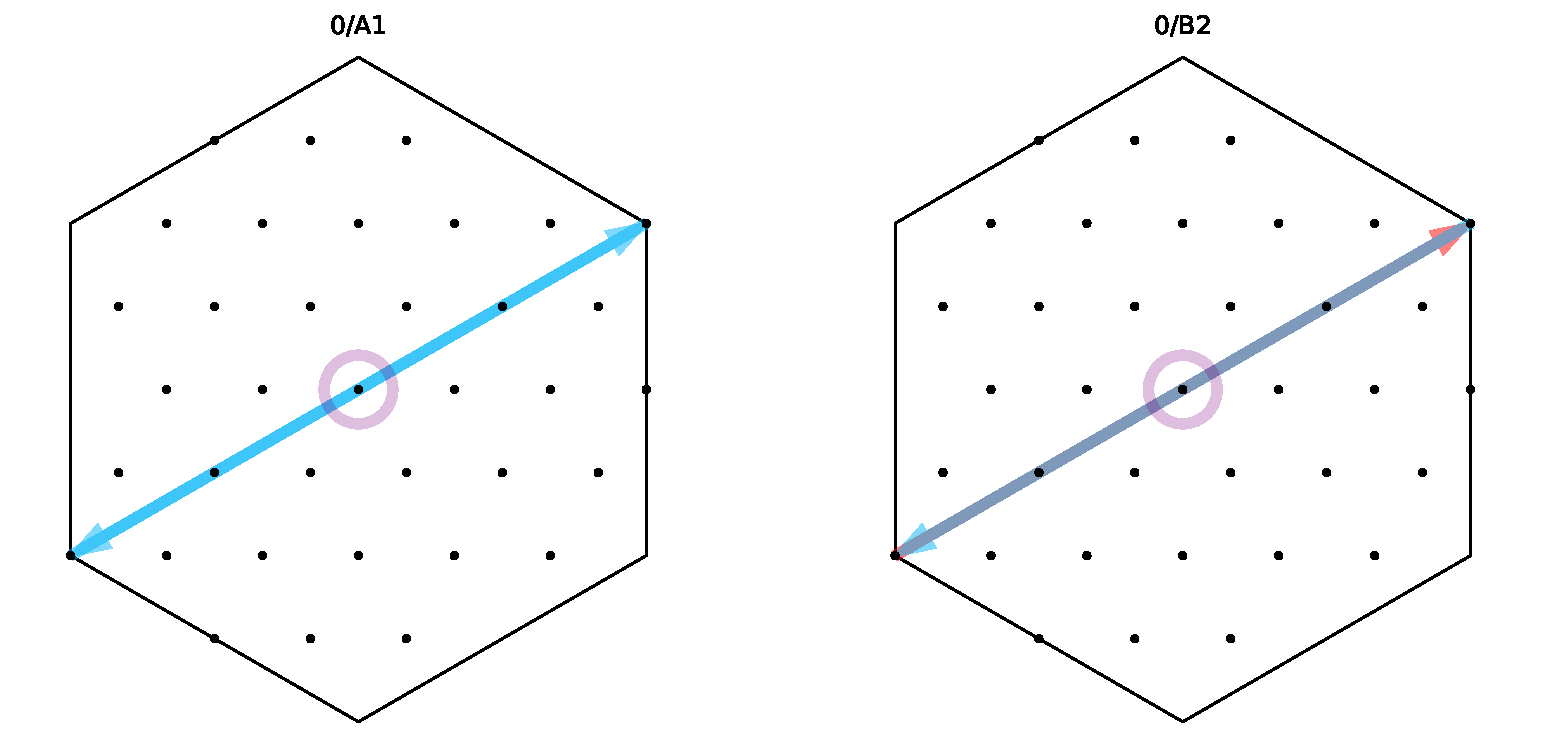
\includegraphics[width=0.5\linewidth]{BZ_used.pdf}}
    \caption{blabla}
    \label{fig:used irrep}
\end{figure}
For simplicity, we will only work at $U = 3.0$ with total momentum $\Gamma$ and source/sink momenta at the Dirac points $K, K'$. The reason is because of data constraints (Table \ref{tab:work_ensembles}) and the available momenta of interest (only $\Gamma, K, K'$ are present for all lattice sizes). This set of momenta gives a constraint on the irreducible representations. We are working only with irreducible representations $A1$ and $B2$ (Figure \ref{fig:used irrep}).

The method for obtaining the binding energy (\ref{eq:binding_energy}) extracts the energy from the two-body correlation function by fitting
\begin{equation}
    f(t) = A\cosh(E_0(t-\frac{\beta}{2})) + C,
    \label{eq:cosh2}
\end{equation}
and then the one-body correlator energy
\begin{equation}
    f(t) = A\cosh(E_0(t-\frac{\beta}{2})),
    \label{eq:cosh1}
\end{equation}
where $A, E_0, C$ are fit parameters for amplitude, ground energy, and a constant that describes the backward propagating. We obtain $\Delta E$ after subtracting the energies. The data analysis then proceeds by reaching the continuum and infinite volume limits.
\begin{figure}
    \begin{subfigure}{.5\textwidth}
      \centering
      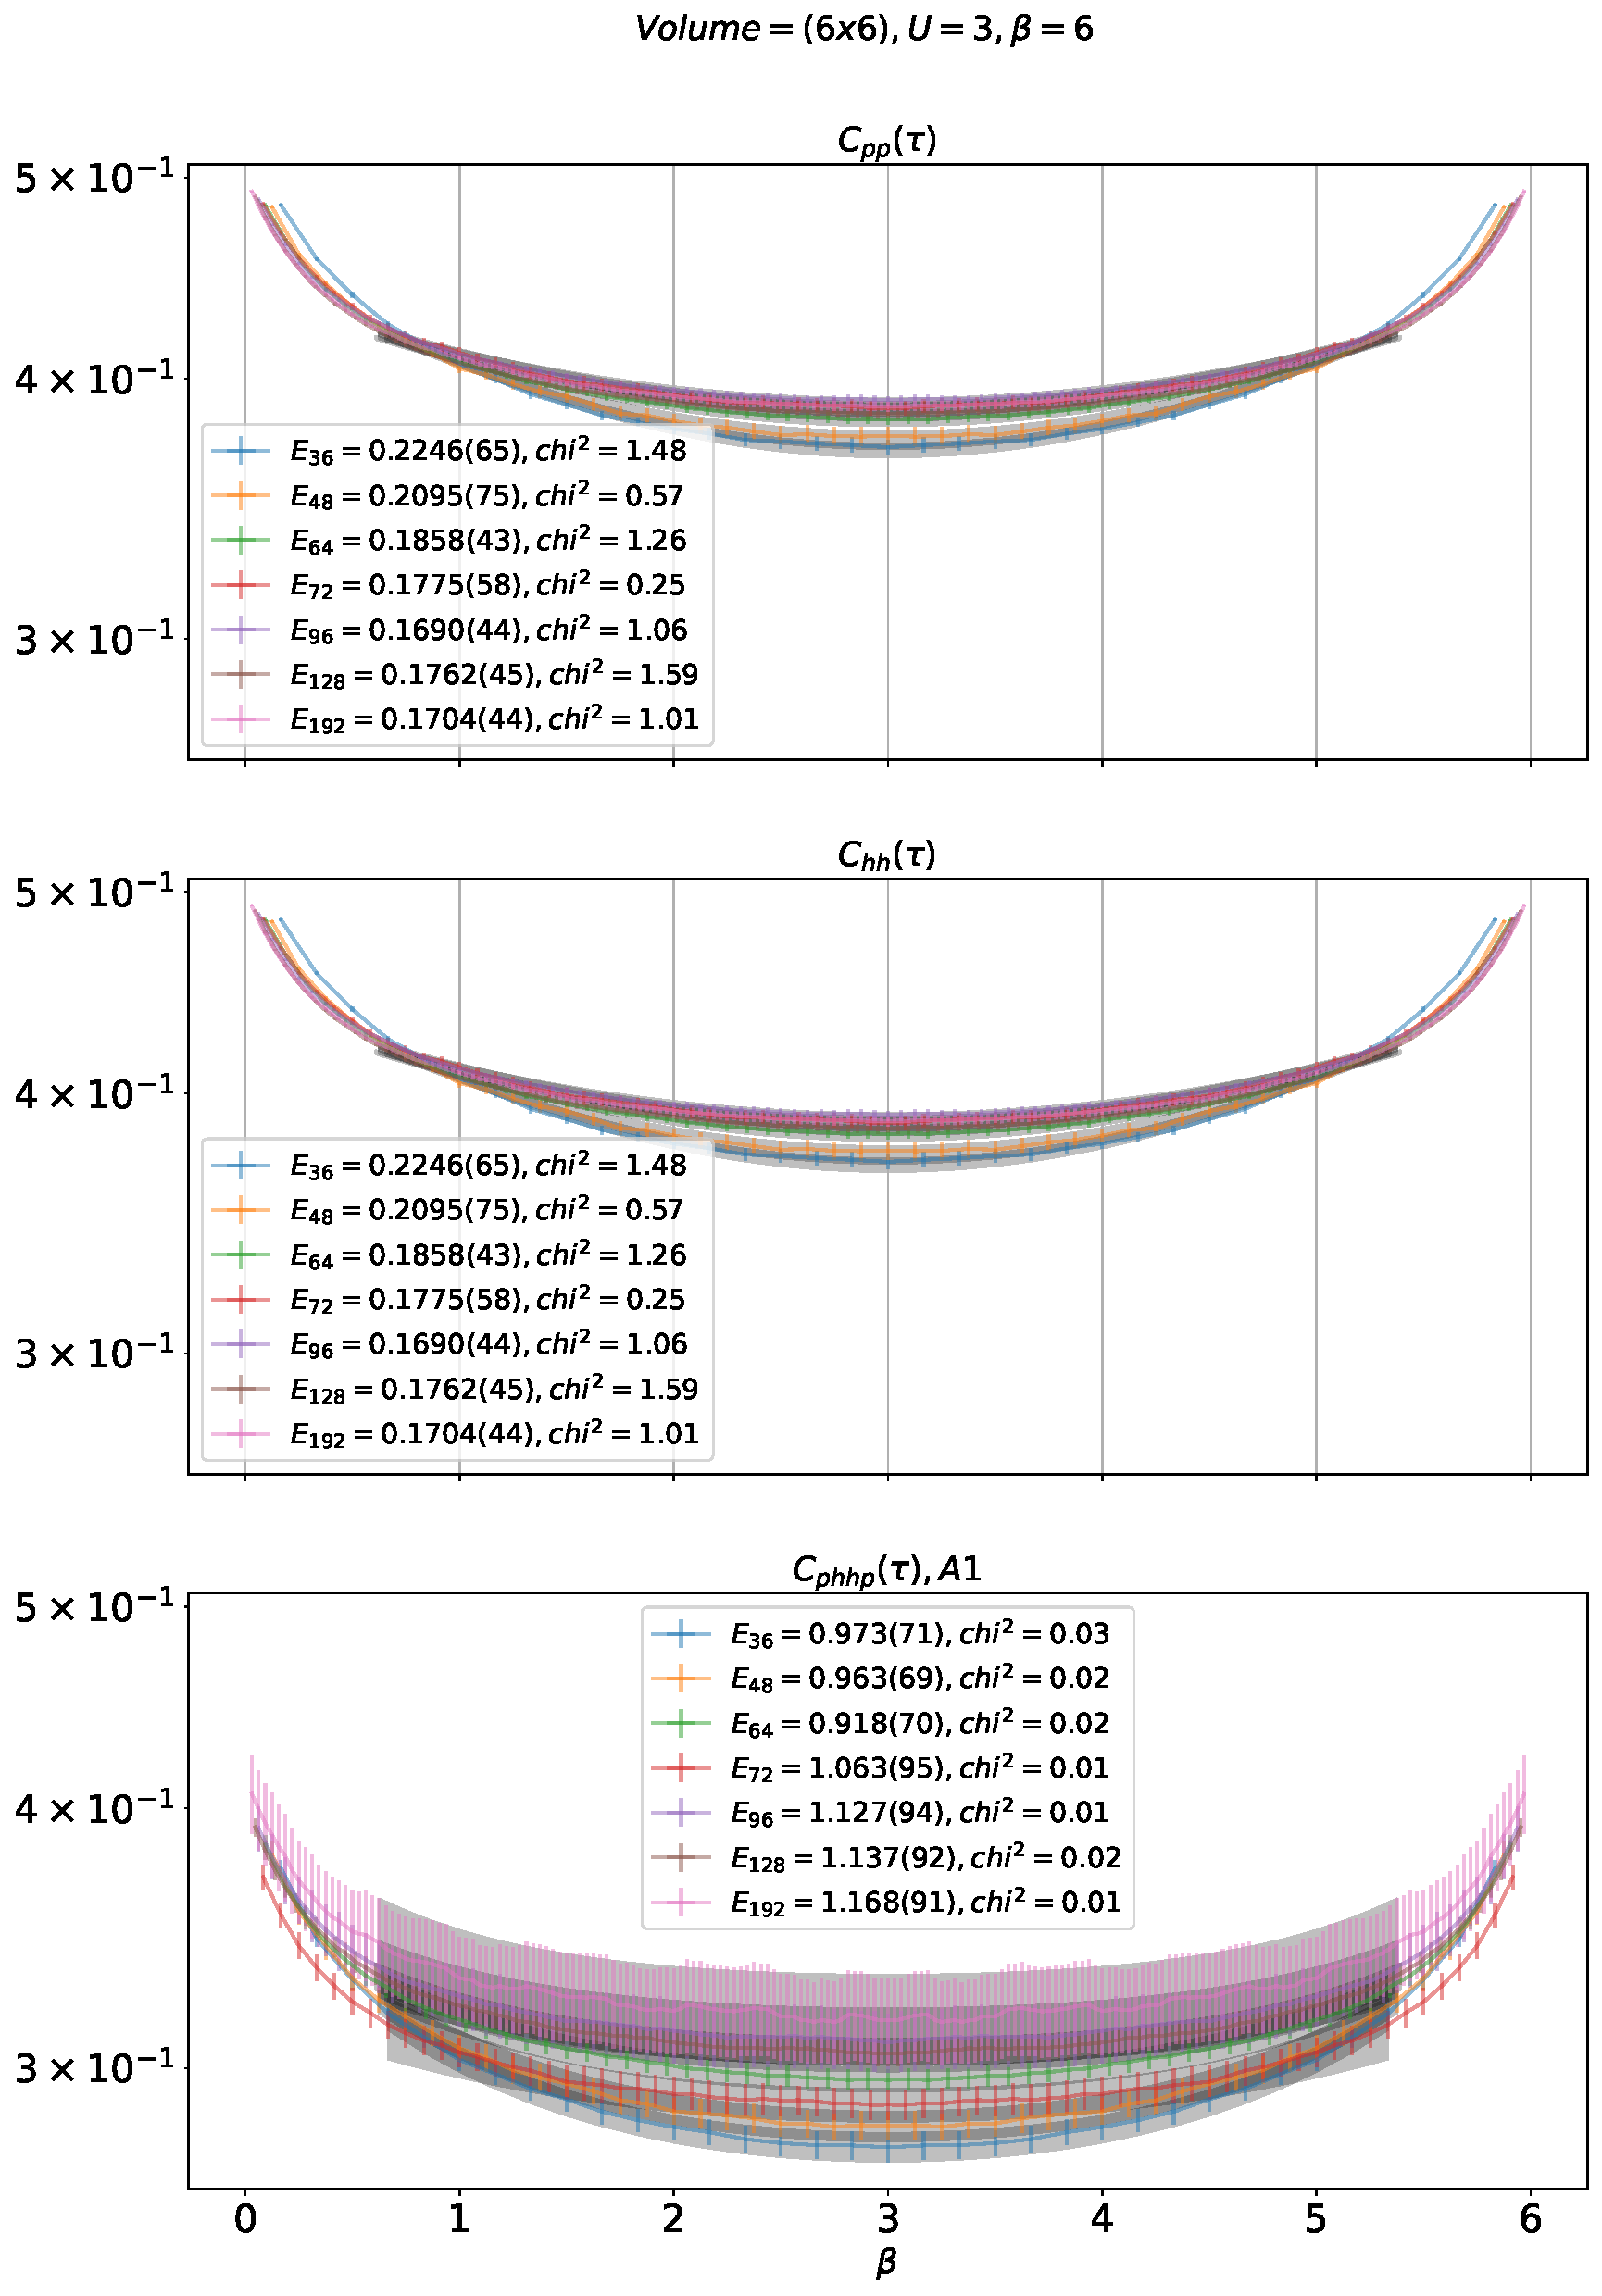
\includegraphics[width=\linewidth]{phhp-0-A1_6x6_U3.0_B6.0.pdf}
    \end{subfigure}%
    \begin{subfigure}{.5\textwidth}
      \centering
      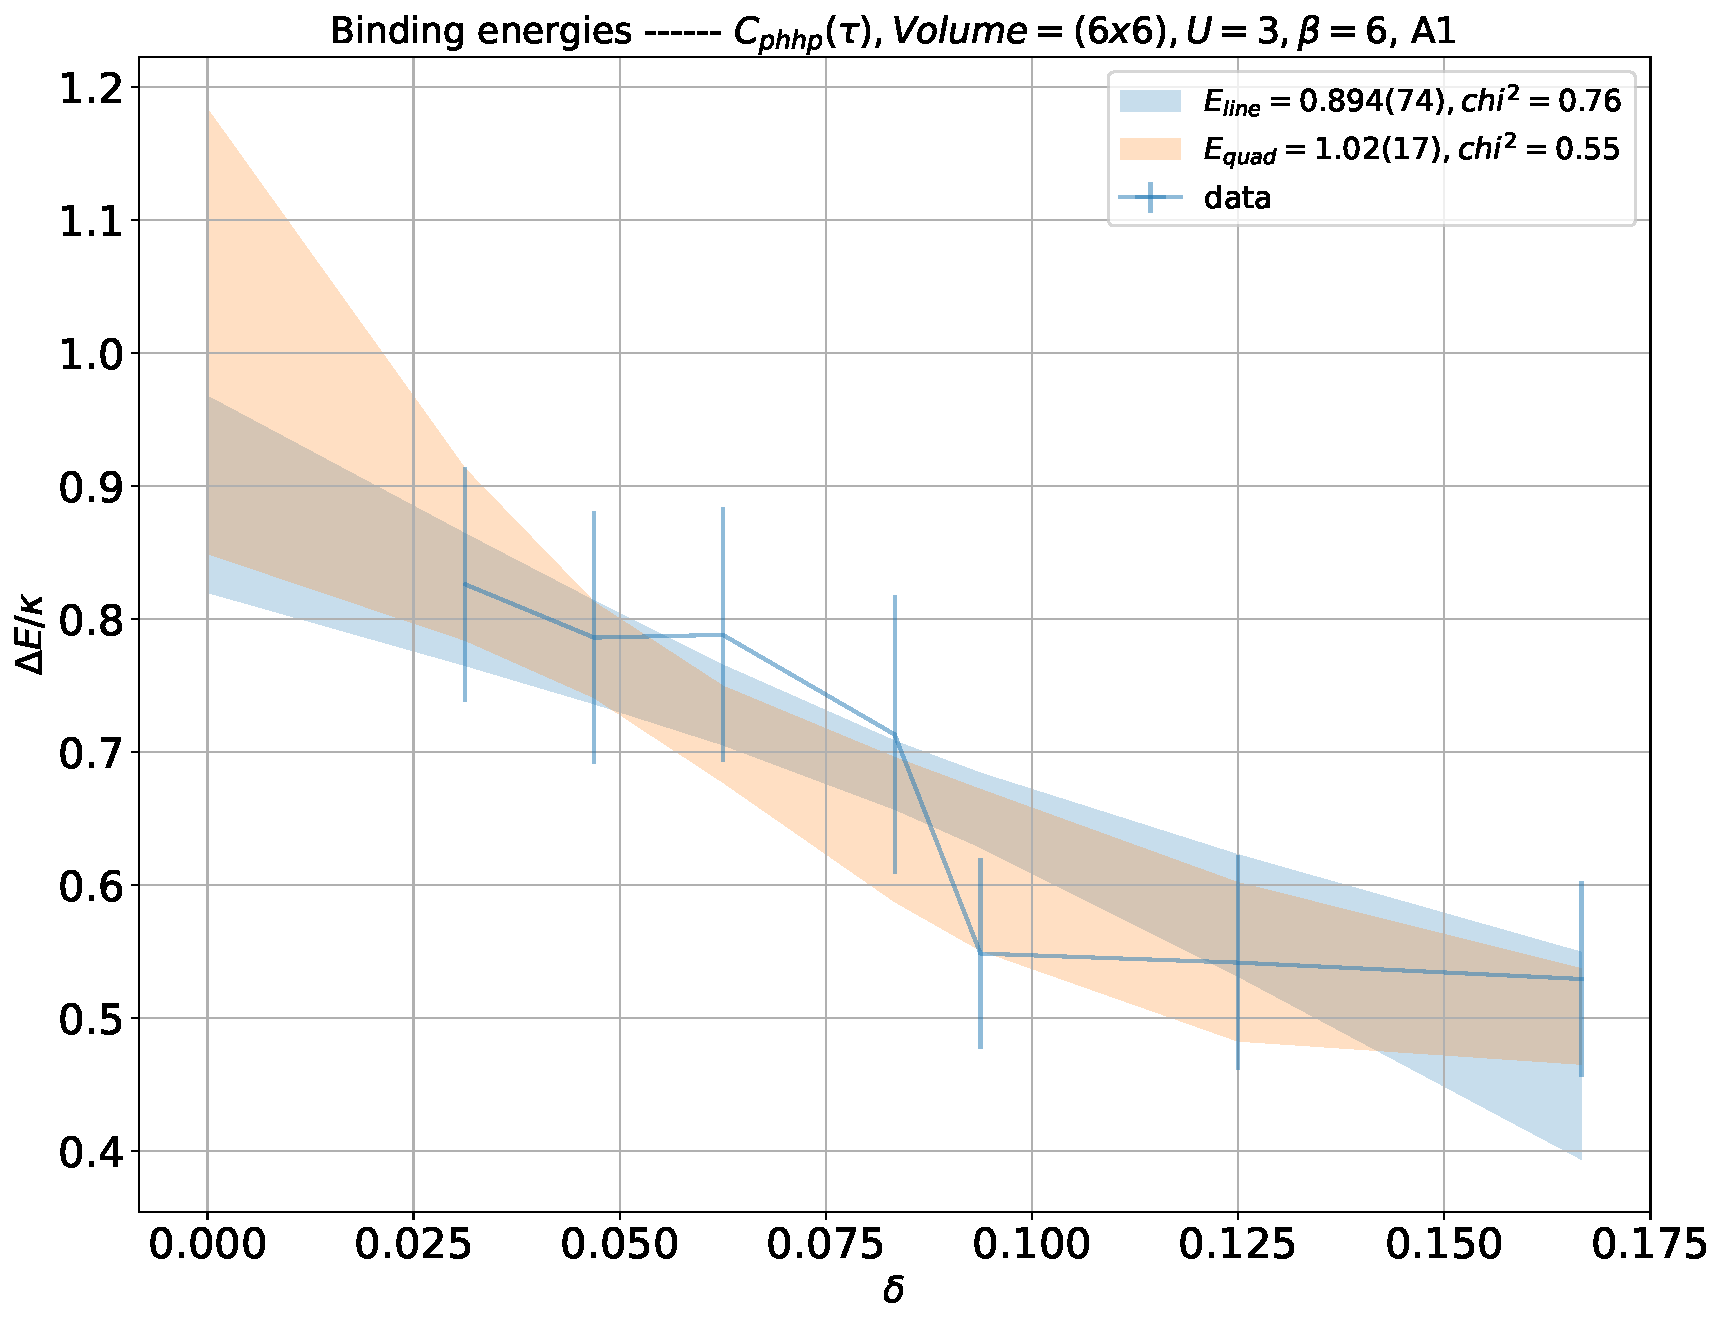
\includegraphics[width=\linewidth]{phhp-0-A1_6x6_U3.0_B6.0_cont.pdf}
    \end{subfigure}
    \caption{plots of....}
    \label{fig:cont_lim}
\end{figure}
It is shown on Figure \ref{fig:cont_lim}, the fitting of (\ref{eq:cosh1}) and (\ref{eq:cosh2}) to one- and two-body correlation functions for all available $N_t$. After that all energies are used to extrapolate to continuum limit using a linear and a quadratic functions. This process is repeated for every lattice size, two-body correlation functions, and irreducible representations (All fits could be seen in Appendix \ref{app:limit}).
\begin{figure}
    \begin{subfigure}{.5\textwidth}
      \centering
      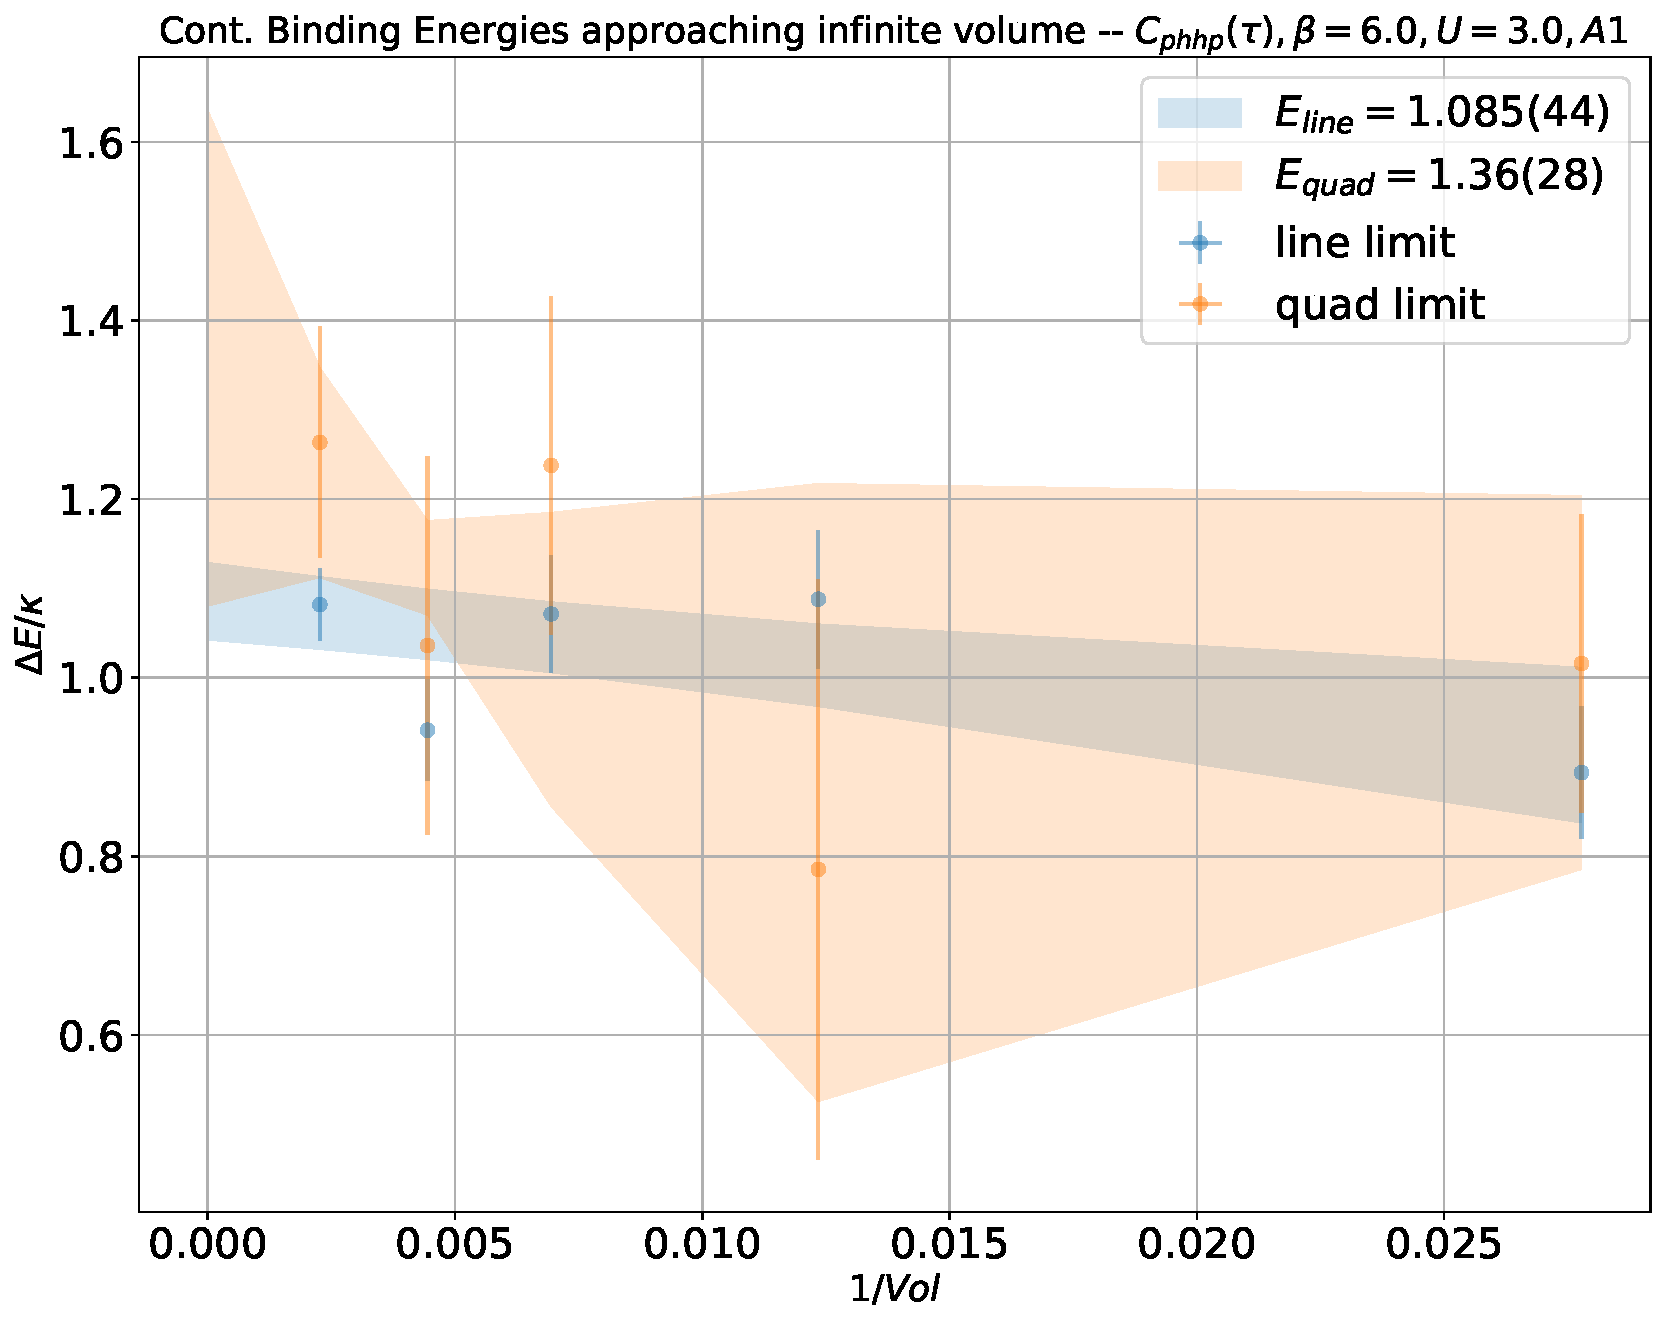
\includegraphics[width=\linewidth]{phhp-0-A1_21x21_U3_B6_vol.pdf}
      \caption{1a}
      \label{fig:sfig1}
    \end{subfigure}%
    \begin{subfigure}{.5\textwidth}
      \centering
      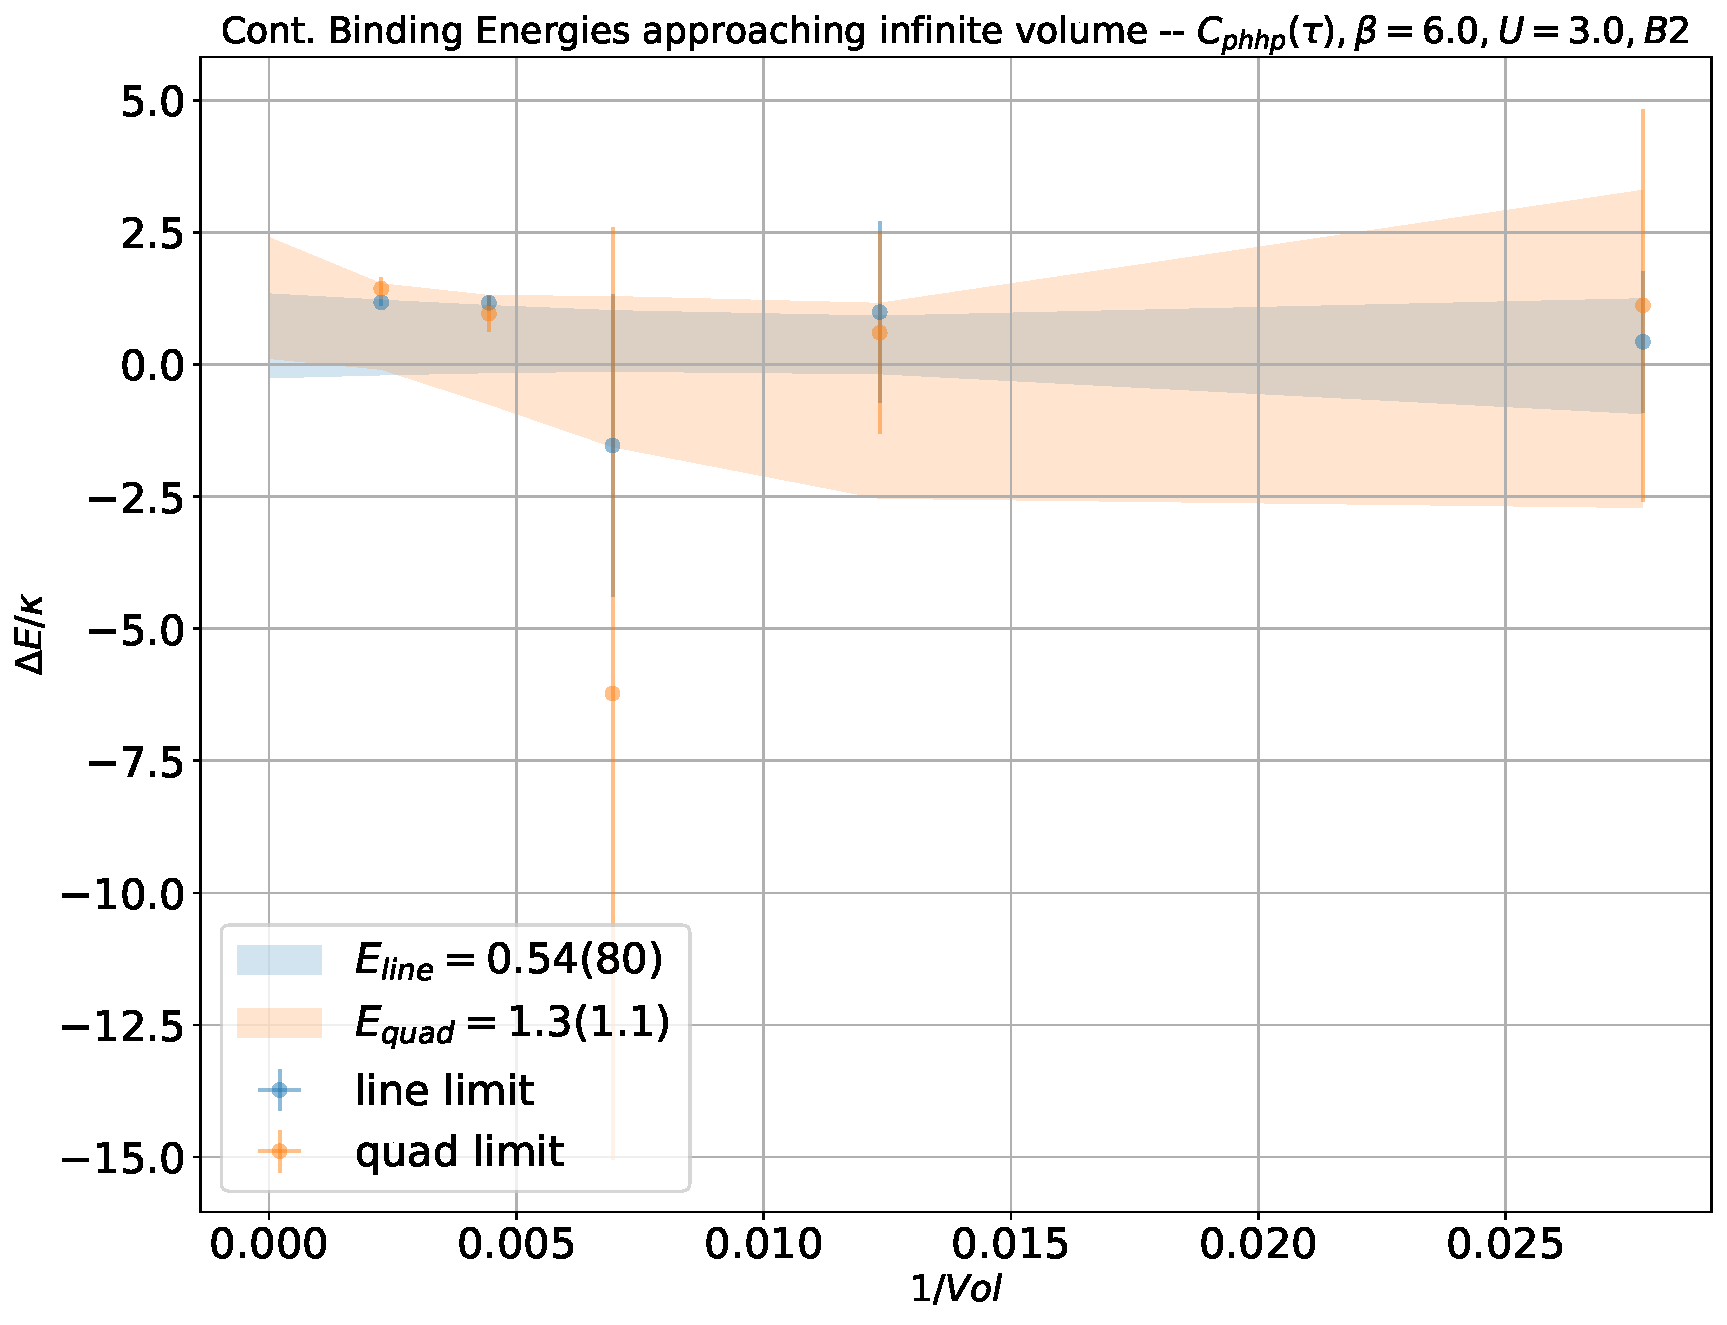
\includegraphics[width=\linewidth]{phhp-0-B2_21x21_U3_B6_vol.pdf}
      \caption{1b}
      \label{fig:sfig2}
    \end{subfigure}
    \begin{subfigure}{.5\textwidth}
        \centering
        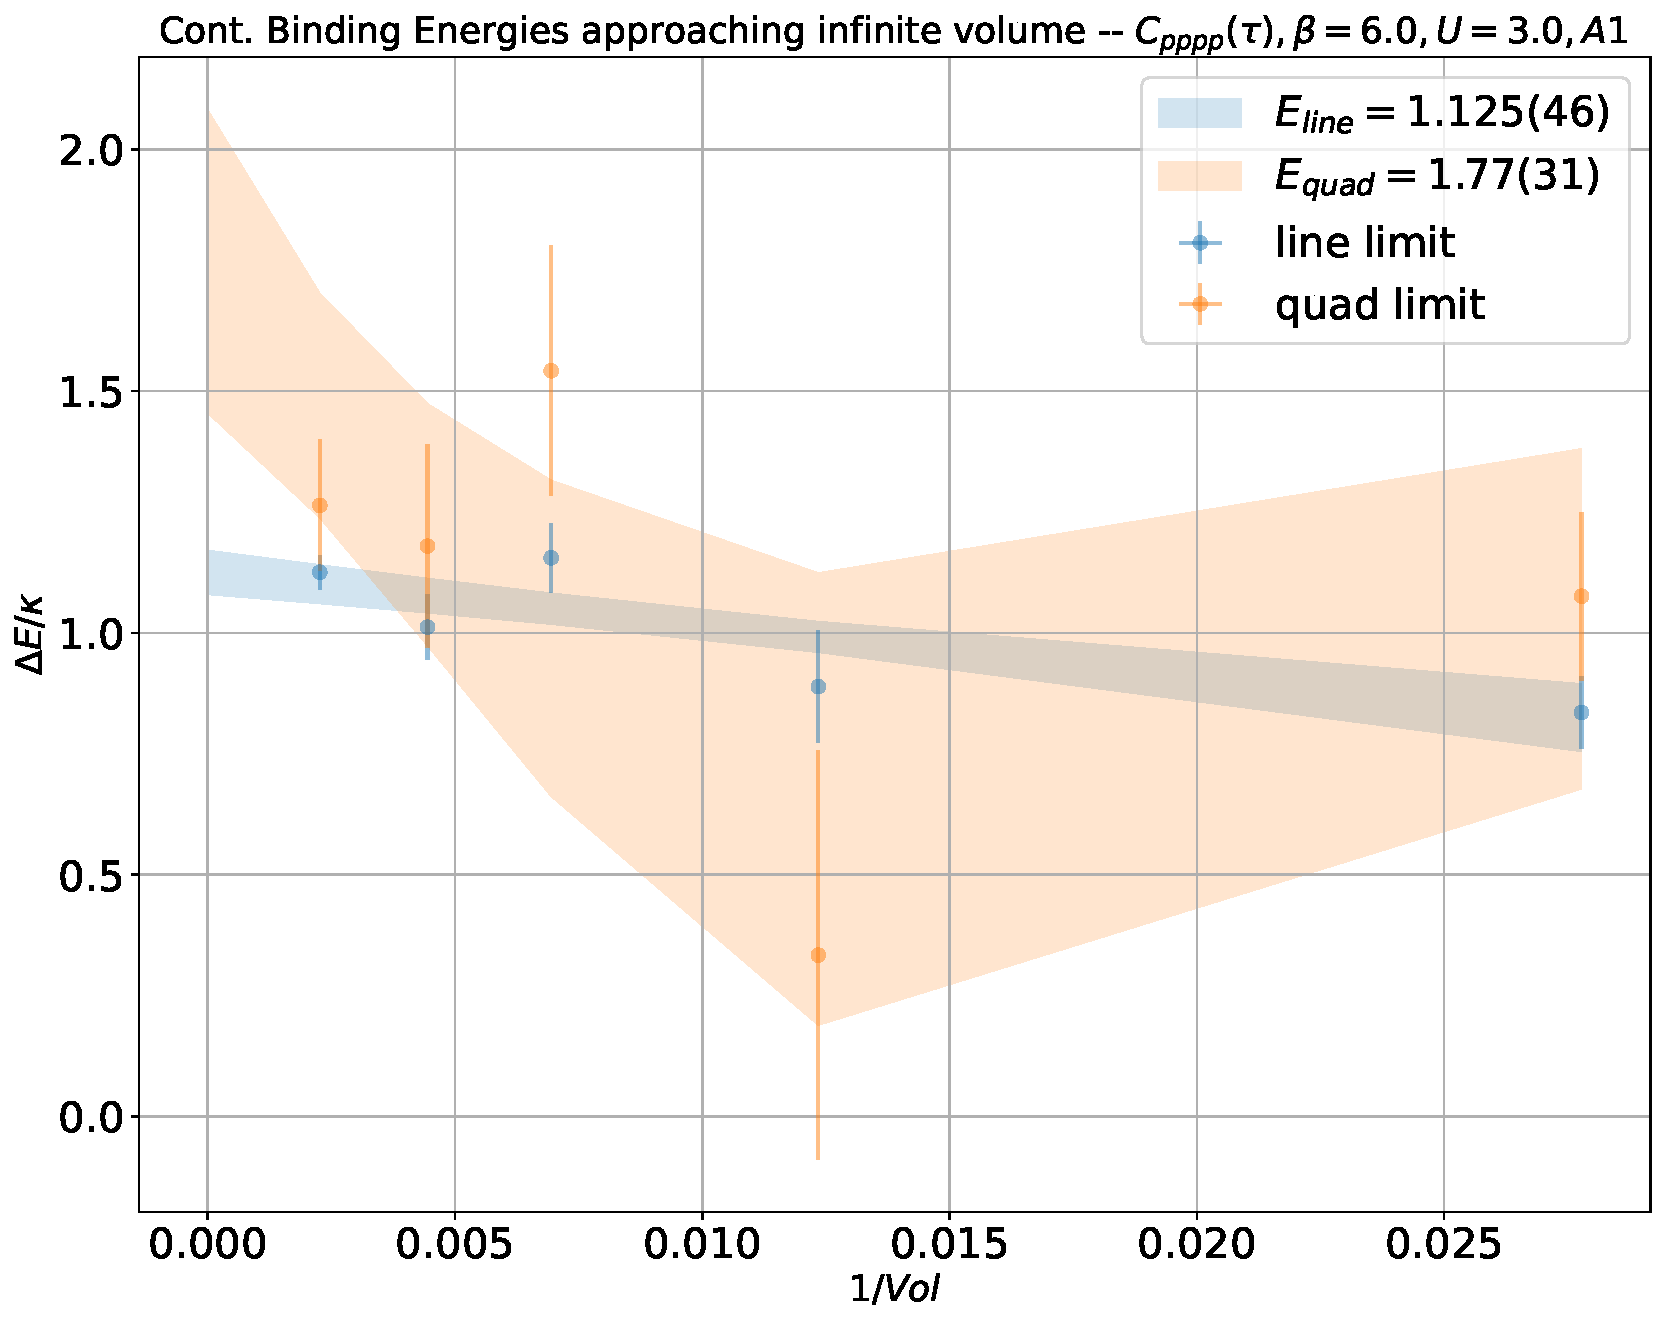
\includegraphics[width=\linewidth]{pppp-0-A1_21x21_U3_B6_vol.pdf}
        \caption{1c}
        \label{fig:sfig3}
    \end{subfigure}
    \begin{subfigure}{.5\textwidth}
        \centering
        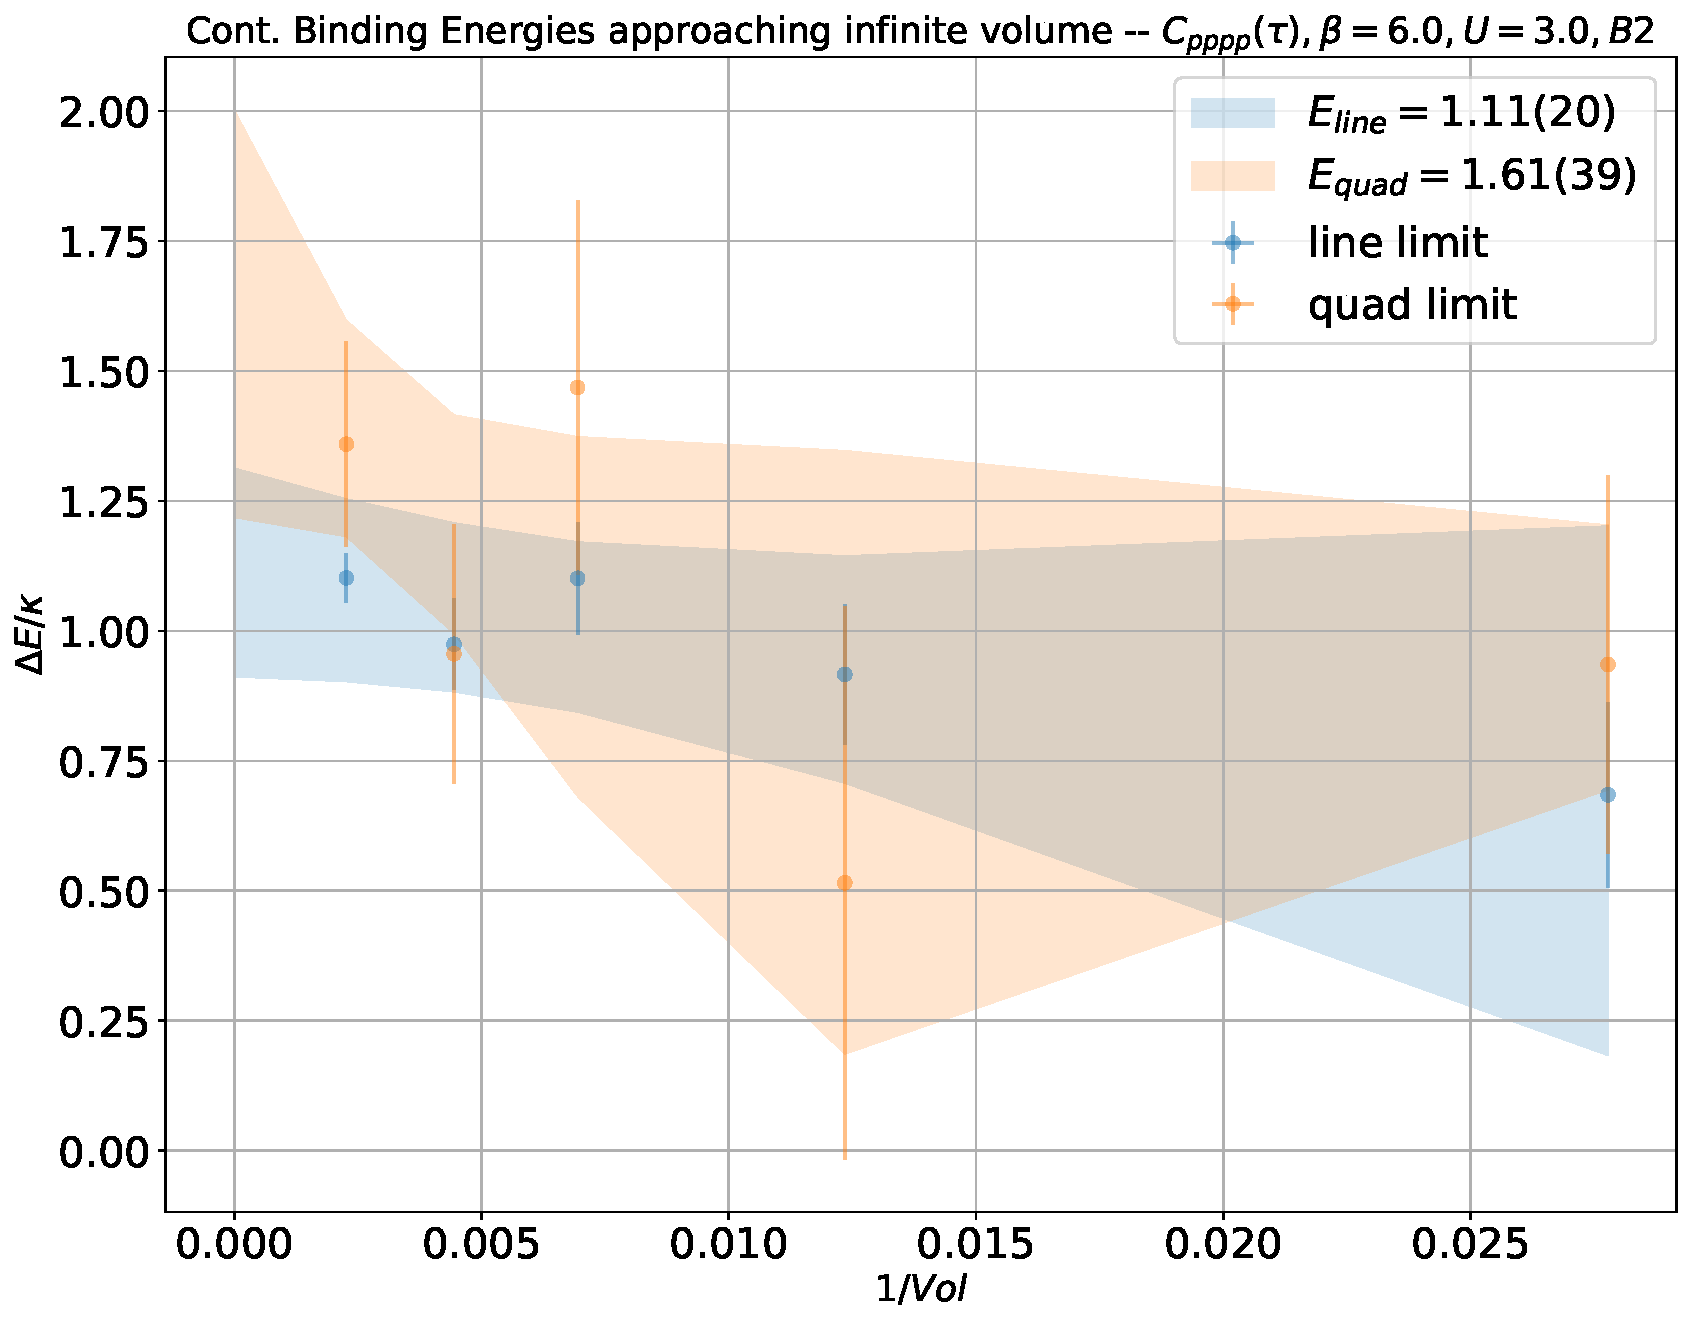
\includegraphics[width=\linewidth]{pppp-0-B2_21x21_U3_B6_vol.pdf}
        \caption{1d}
        \label{fig:sfig4}
    \end{subfigure}
    \caption{plots of....}
    \label{fig:u3vol}
  \end{figure}
The infinite volume results on Figure \ref{fig:u3vol} show that the exciton's binding energy is a positive number for finite temperature and $U=3.0$. Furthermore, the same approximation to the particle-particle correlation functions shows as expected that their binding energy is also positive (Figure \ref{fig:u3vol}). Both irreducible representations have the same behavior.

We note that the results of $\Delta E_{phhp}$ and $\Delta E_{pppp}$ show a small scaling when extrapolating of the infinite volume. This means that we could try to fit and extrapolate our data to the continuum limit followed by the zero temperature limit at finite volume. We can assume that the result we get, is in the vicinity of the true value, but with extra systematic error. From the available ensembles (Table \todo{Add more tables}), we could not only get results for $U=3.0$ but also for $U=4.0$, which is on the other side of the critical coupling $U\approx 3.85$. Here, we will show only the final results for both correlation function at both couplings and irreducible representations. All plots reaching the continuum limit are shown in Appendix \ref{app:limit}. 
\begin{figure}
    \begin{subfigure}{.5\textwidth}
      \centering
      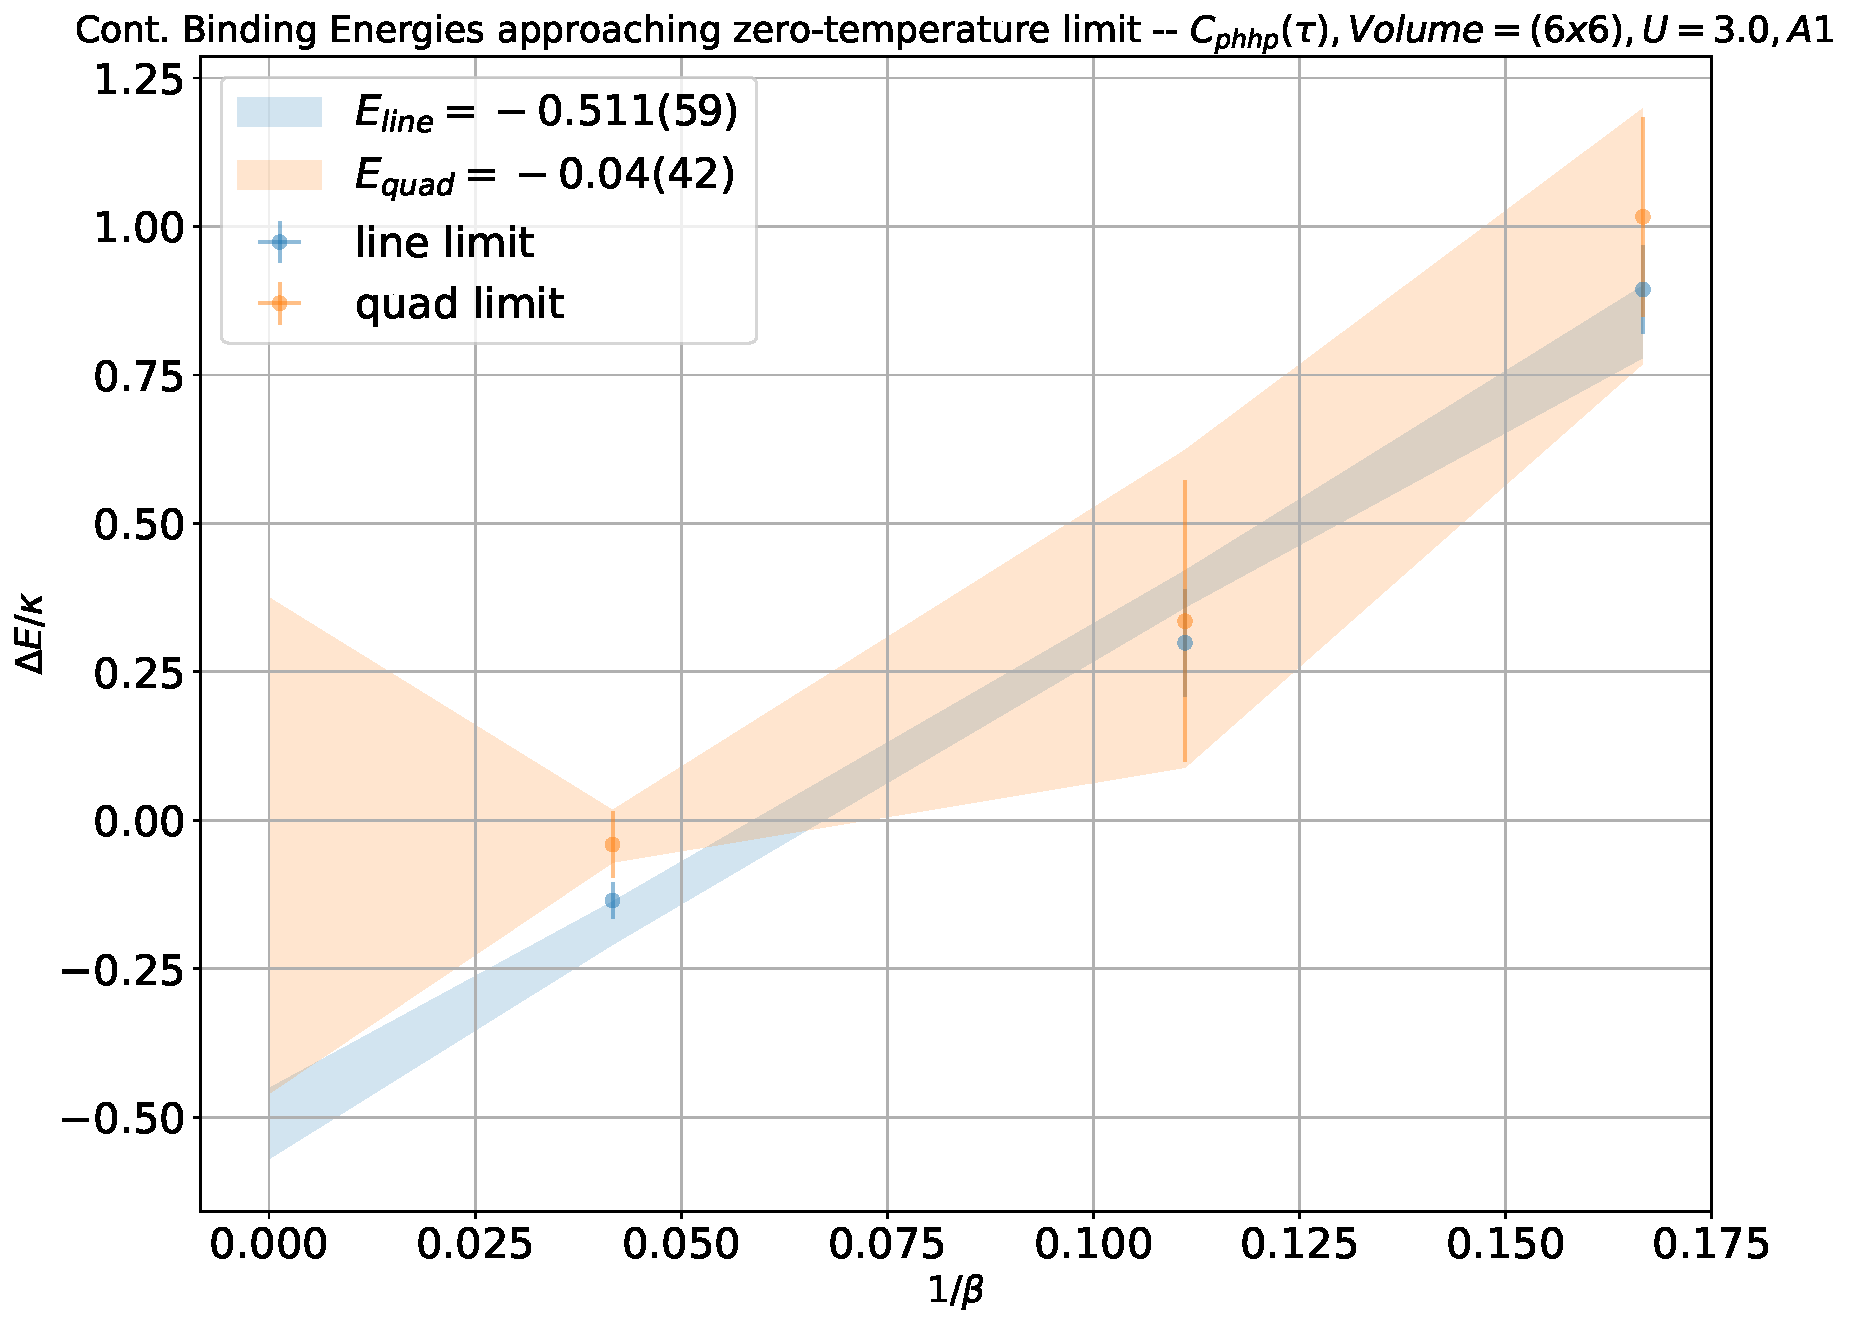
\includegraphics[width=\linewidth]{phhp-0-A1_6x6_U3.0_B24.0_temp.pdf}
      \caption{1a}
      \label{fig:sfig1}
    \end{subfigure}%
    \begin{subfigure}{.5\textwidth}
      \centering
      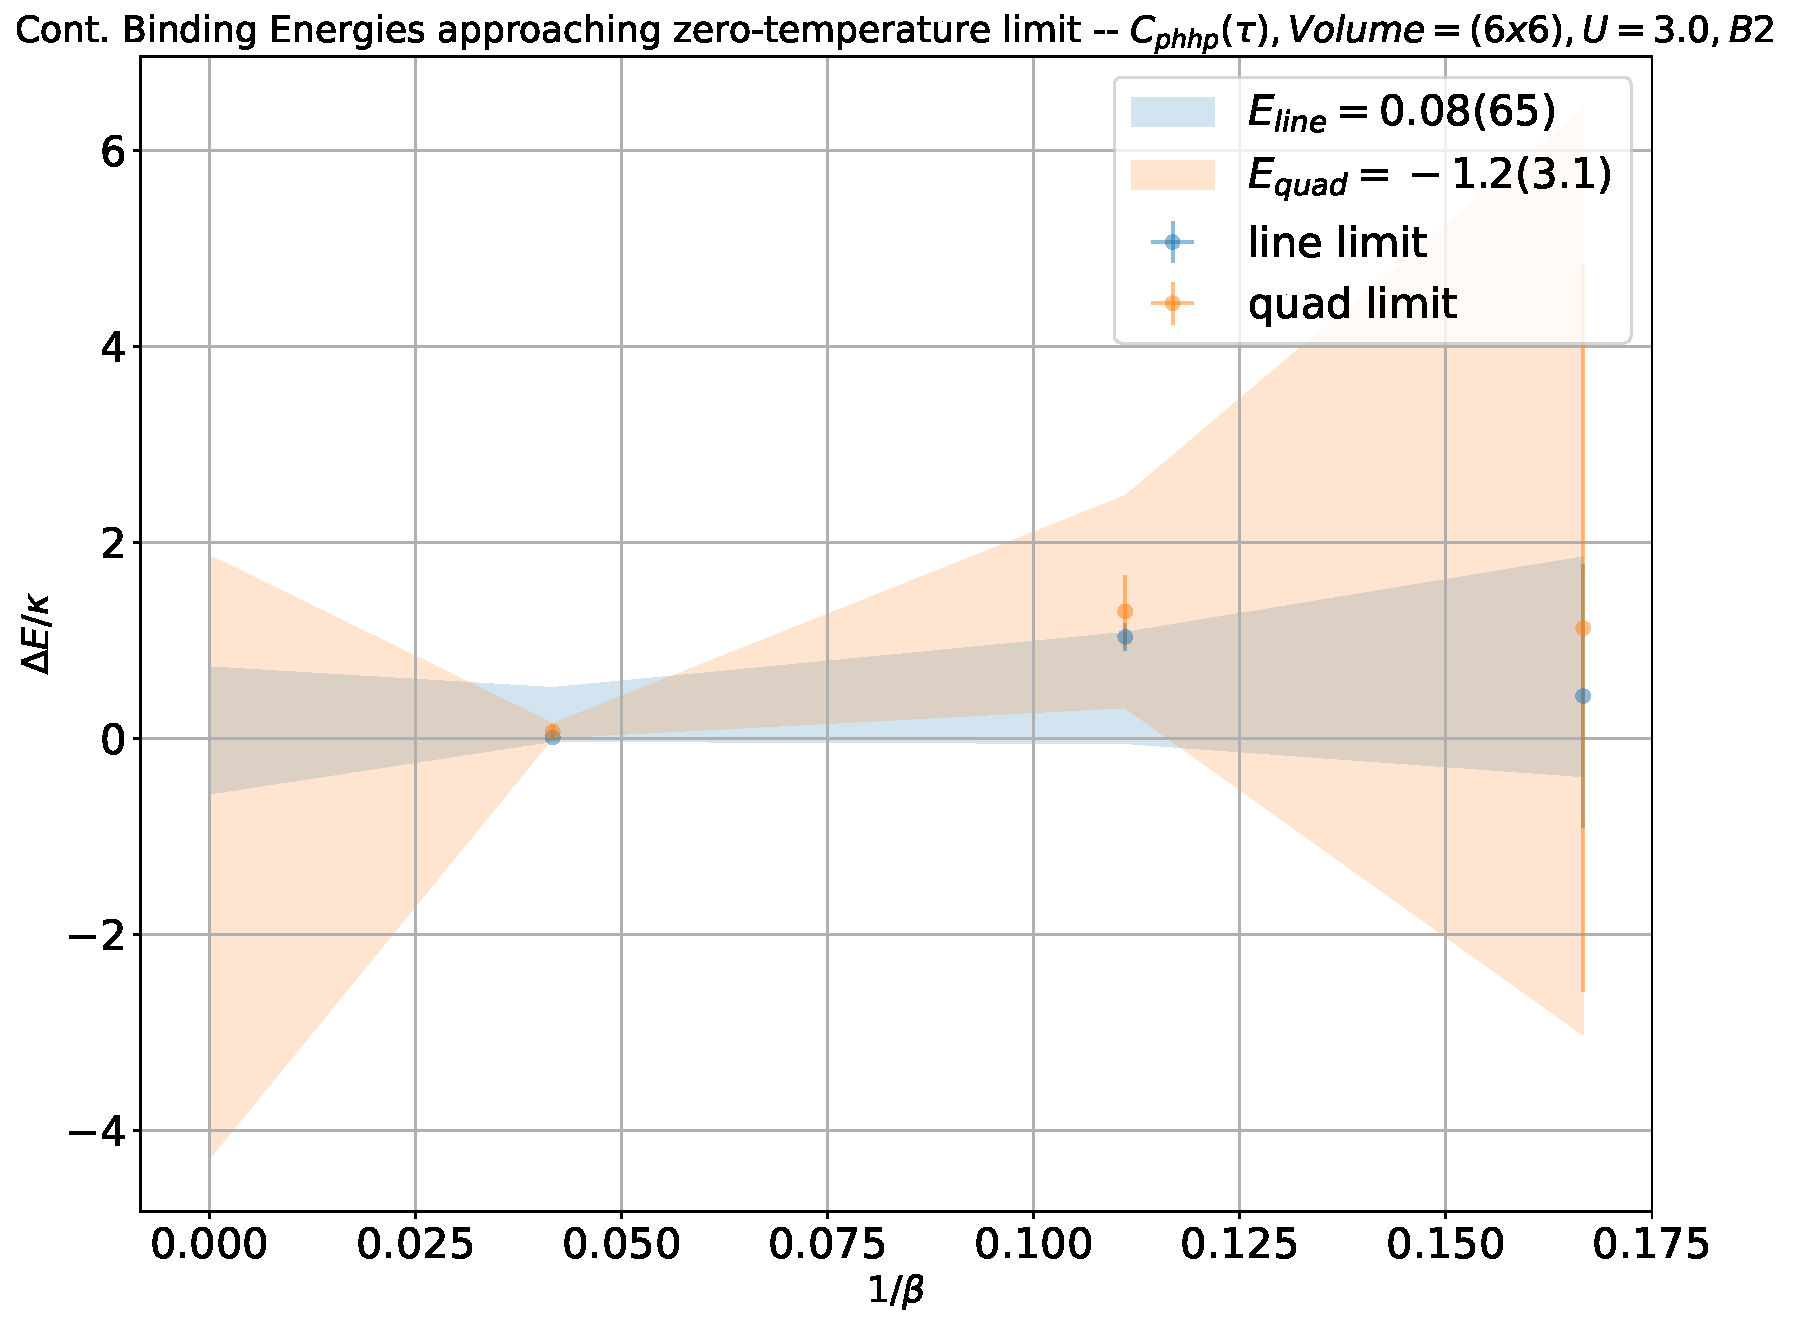
\includegraphics[width=\linewidth]{phhp-0-B2_6x6_U3.0_B24.0_temp.pdf}
      \caption{1b}
      \label{fig:sfig2}
    \end{subfigure}
    \begin{subfigure}{.5\textwidth}
        \centering
        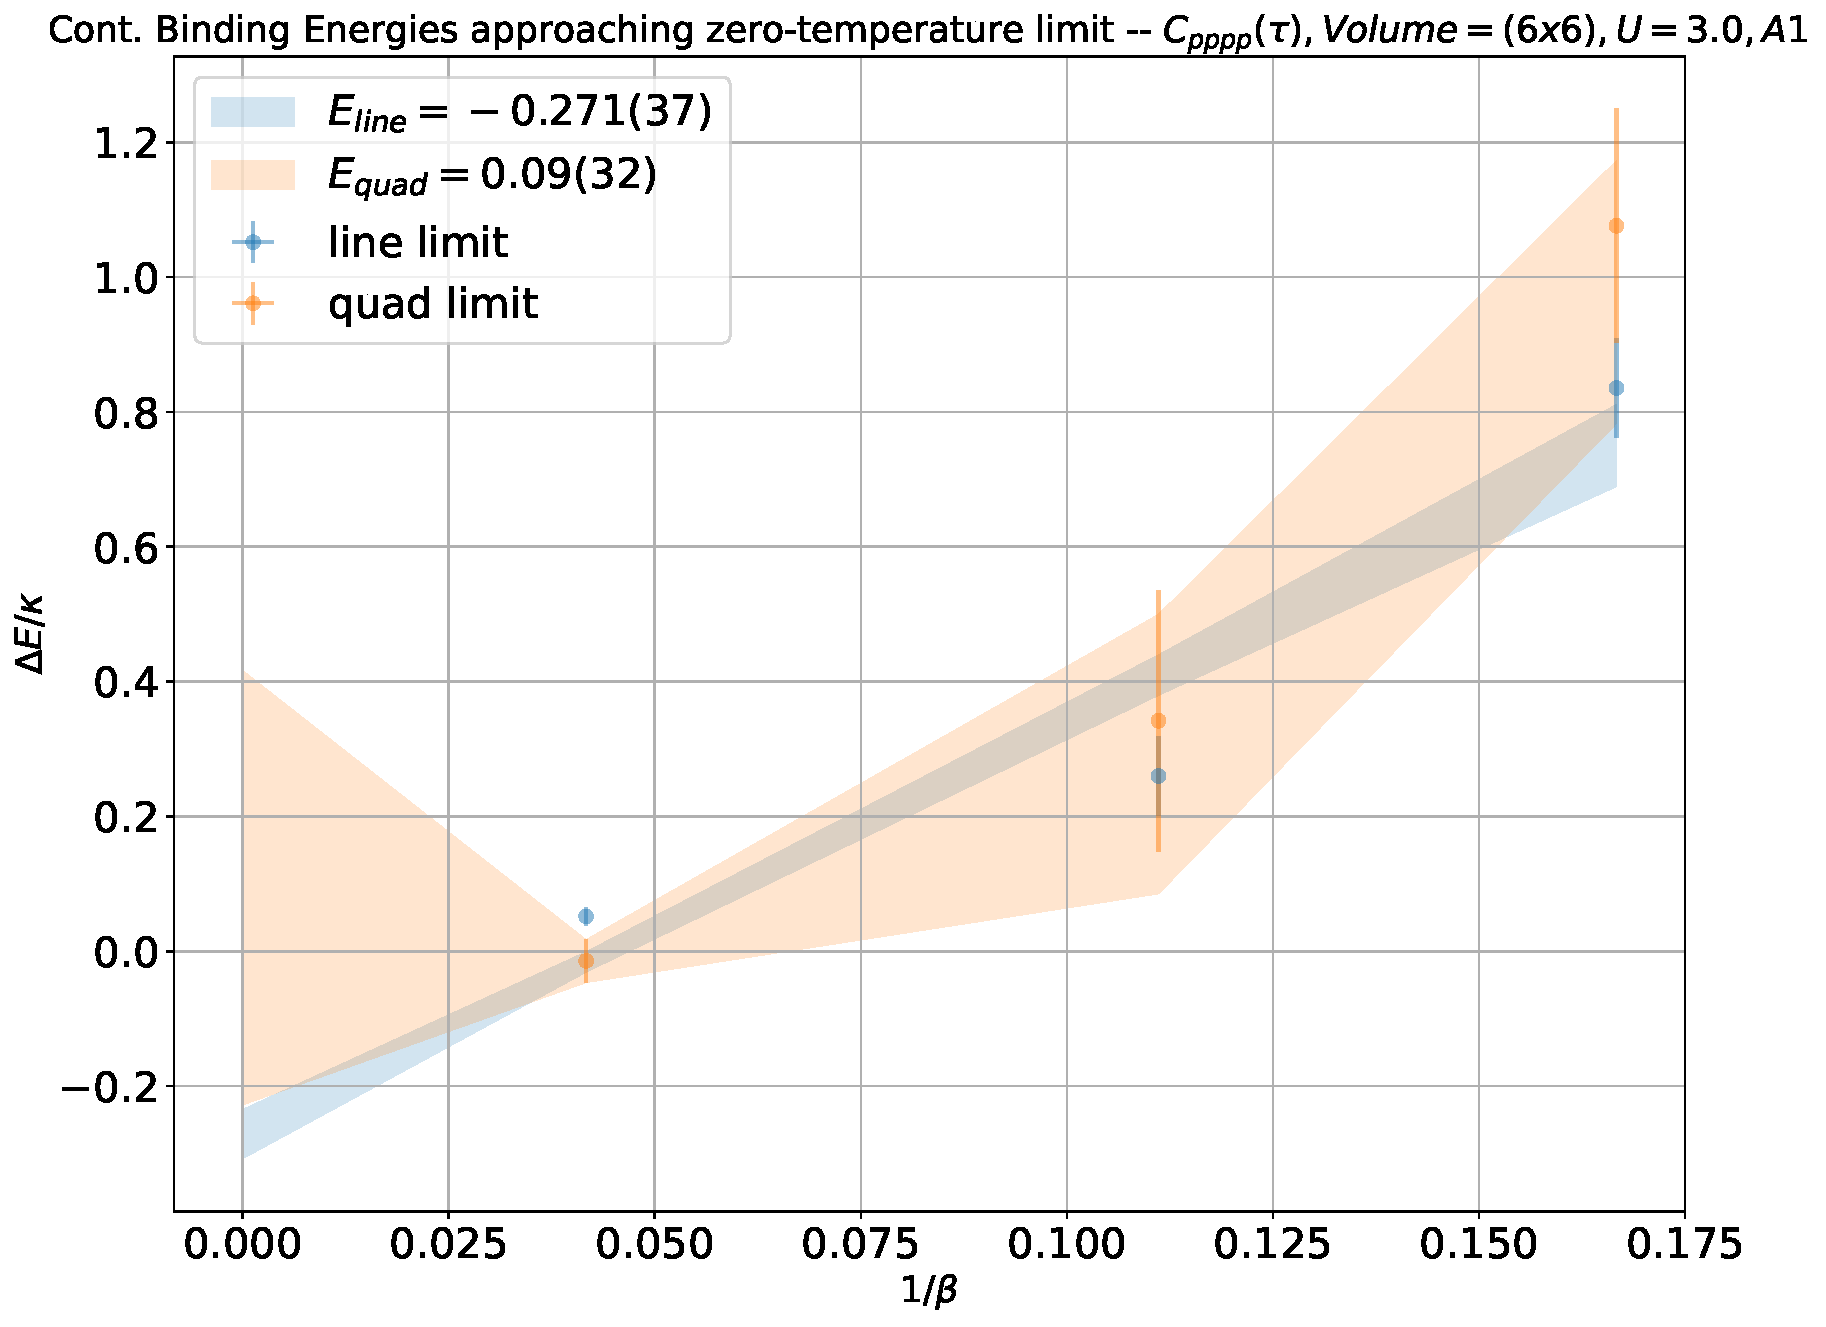
\includegraphics[width=\linewidth]{pppp-0-A1_6x6_U3.0_B24.0_temp.pdf}
        \caption{1c}
        \label{fig:sfig3}
    \end{subfigure}
    \begin{subfigure}{.5\textwidth}
        \centering
        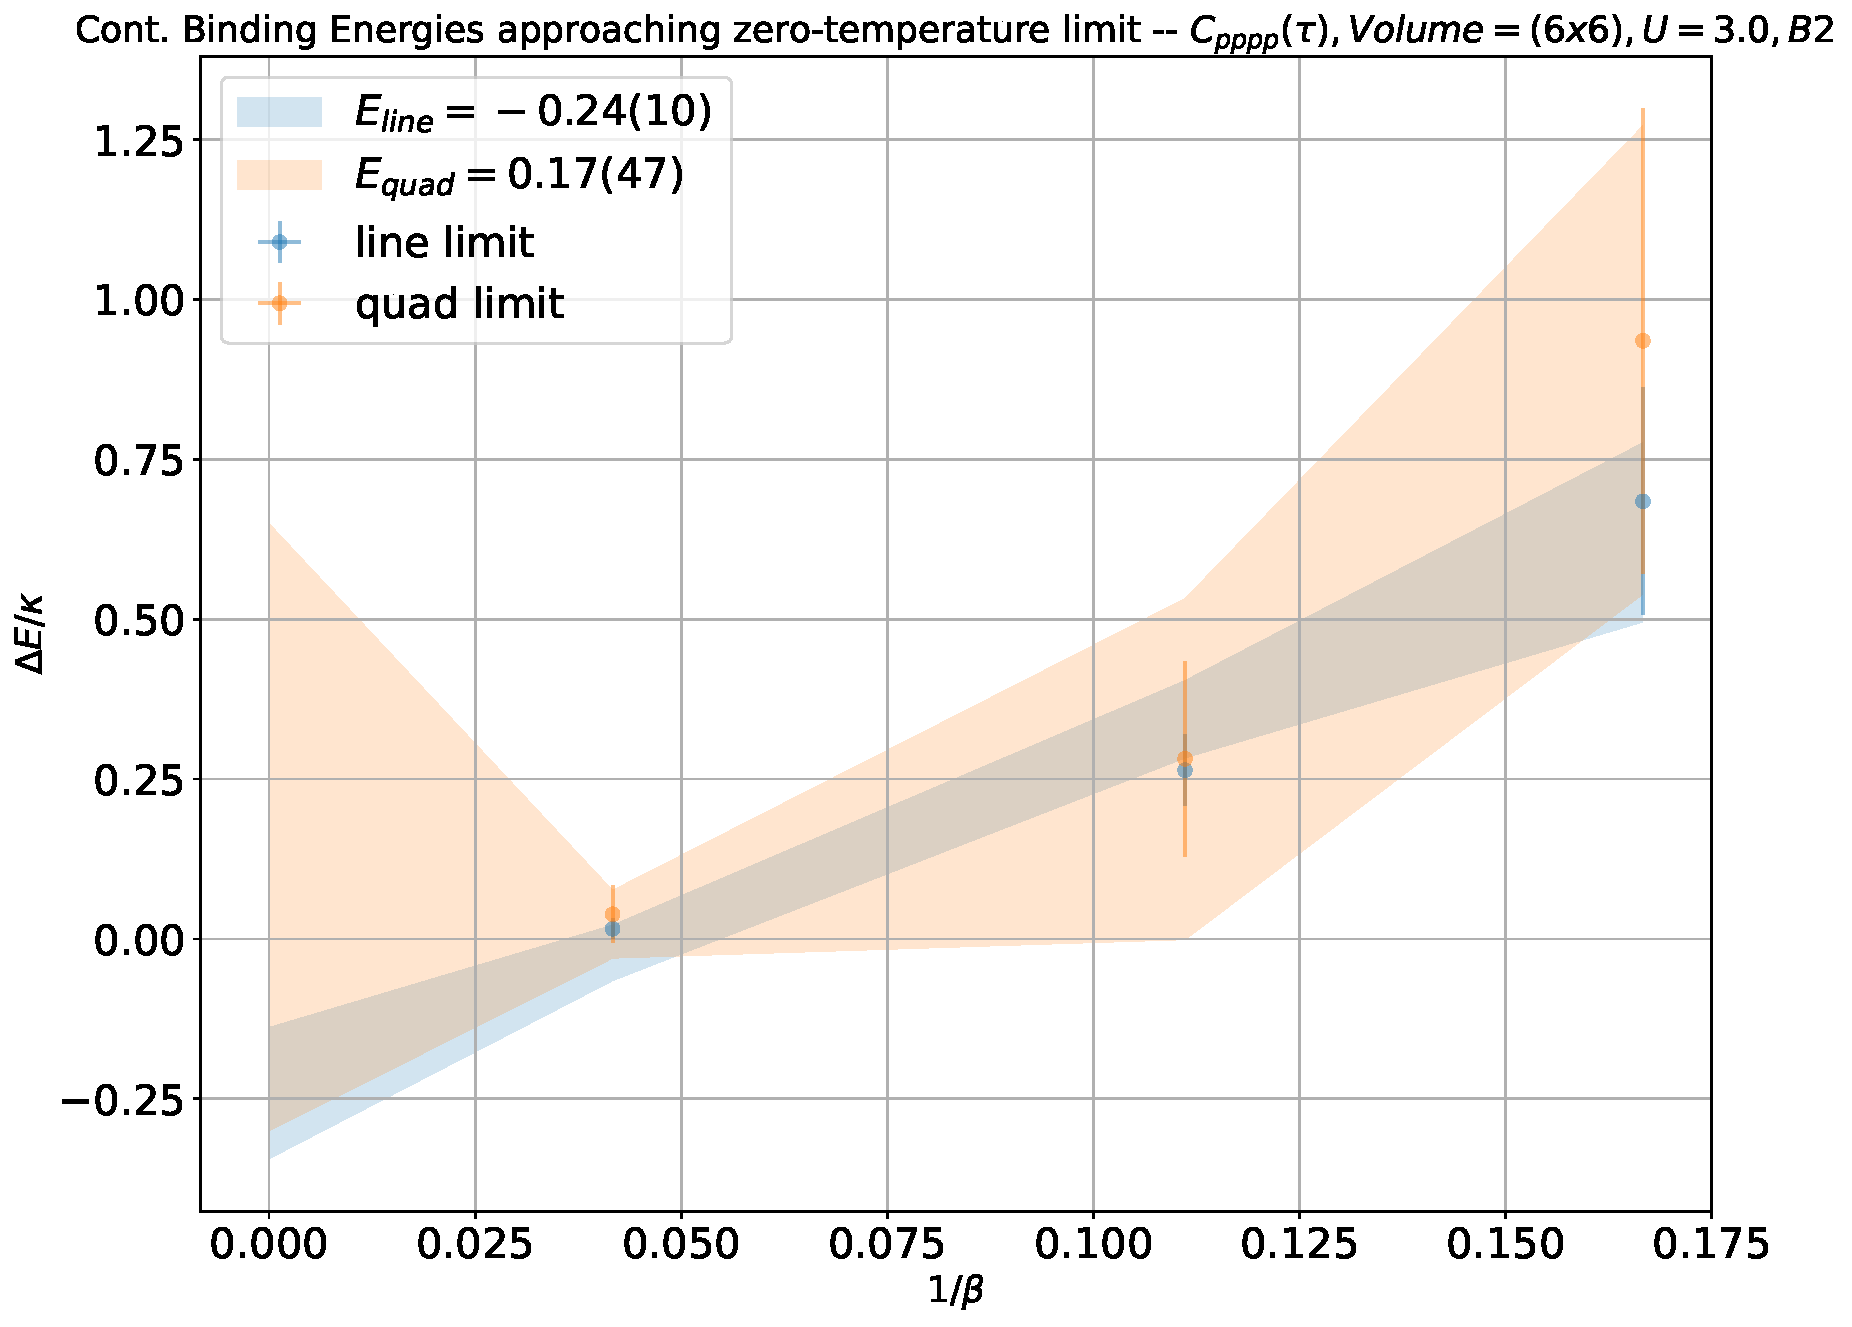
\includegraphics[width=\linewidth]{pppp-0-B2_6x6_U3.0_B24.0_temp.pdf}
        \caption{1d}
        \label{fig:sfig4}
    \end{subfigure}
    \caption{plots of....}
    \label{fig:u3temp}
  \end{figure}
The results for $U=3.0$ (Figure \ref{fig:u3temp}) show that the binding energy of the exciton as well as the particle pair is close to zero for both irreducible representations (Figure \ref{fig:u4temp}). 
\begin{figure}
    \begin{subfigure}{.5\textwidth}
      \centering
      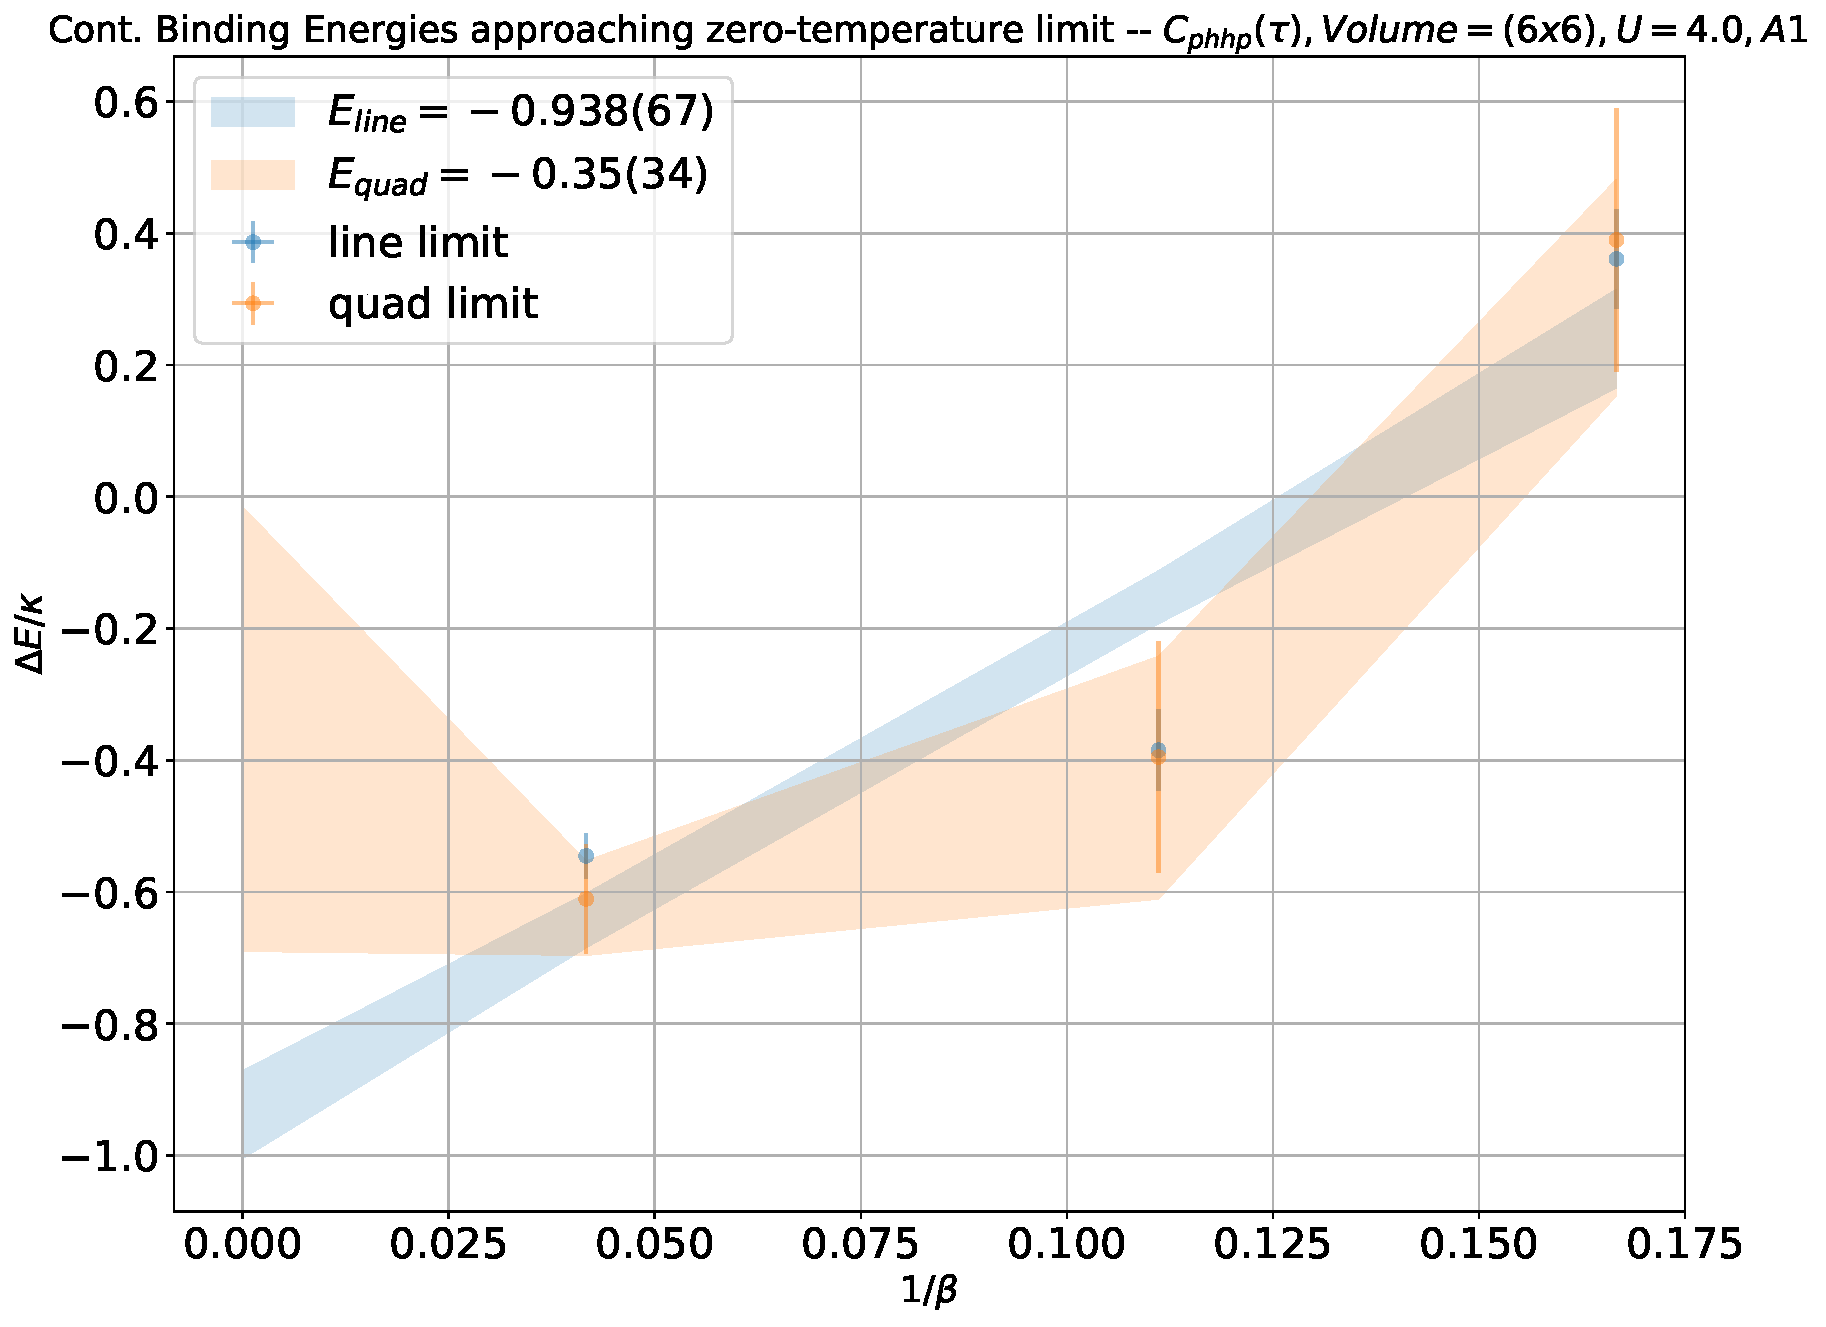
\includegraphics[width=\linewidth]{phhp-0-A1_6x6_U4.0_B24.0_temp.pdf}
      \caption{1a}
      \label{fig:sfig1}
    \end{subfigure}%
    \begin{subfigure}{.5\textwidth}
      \centering
      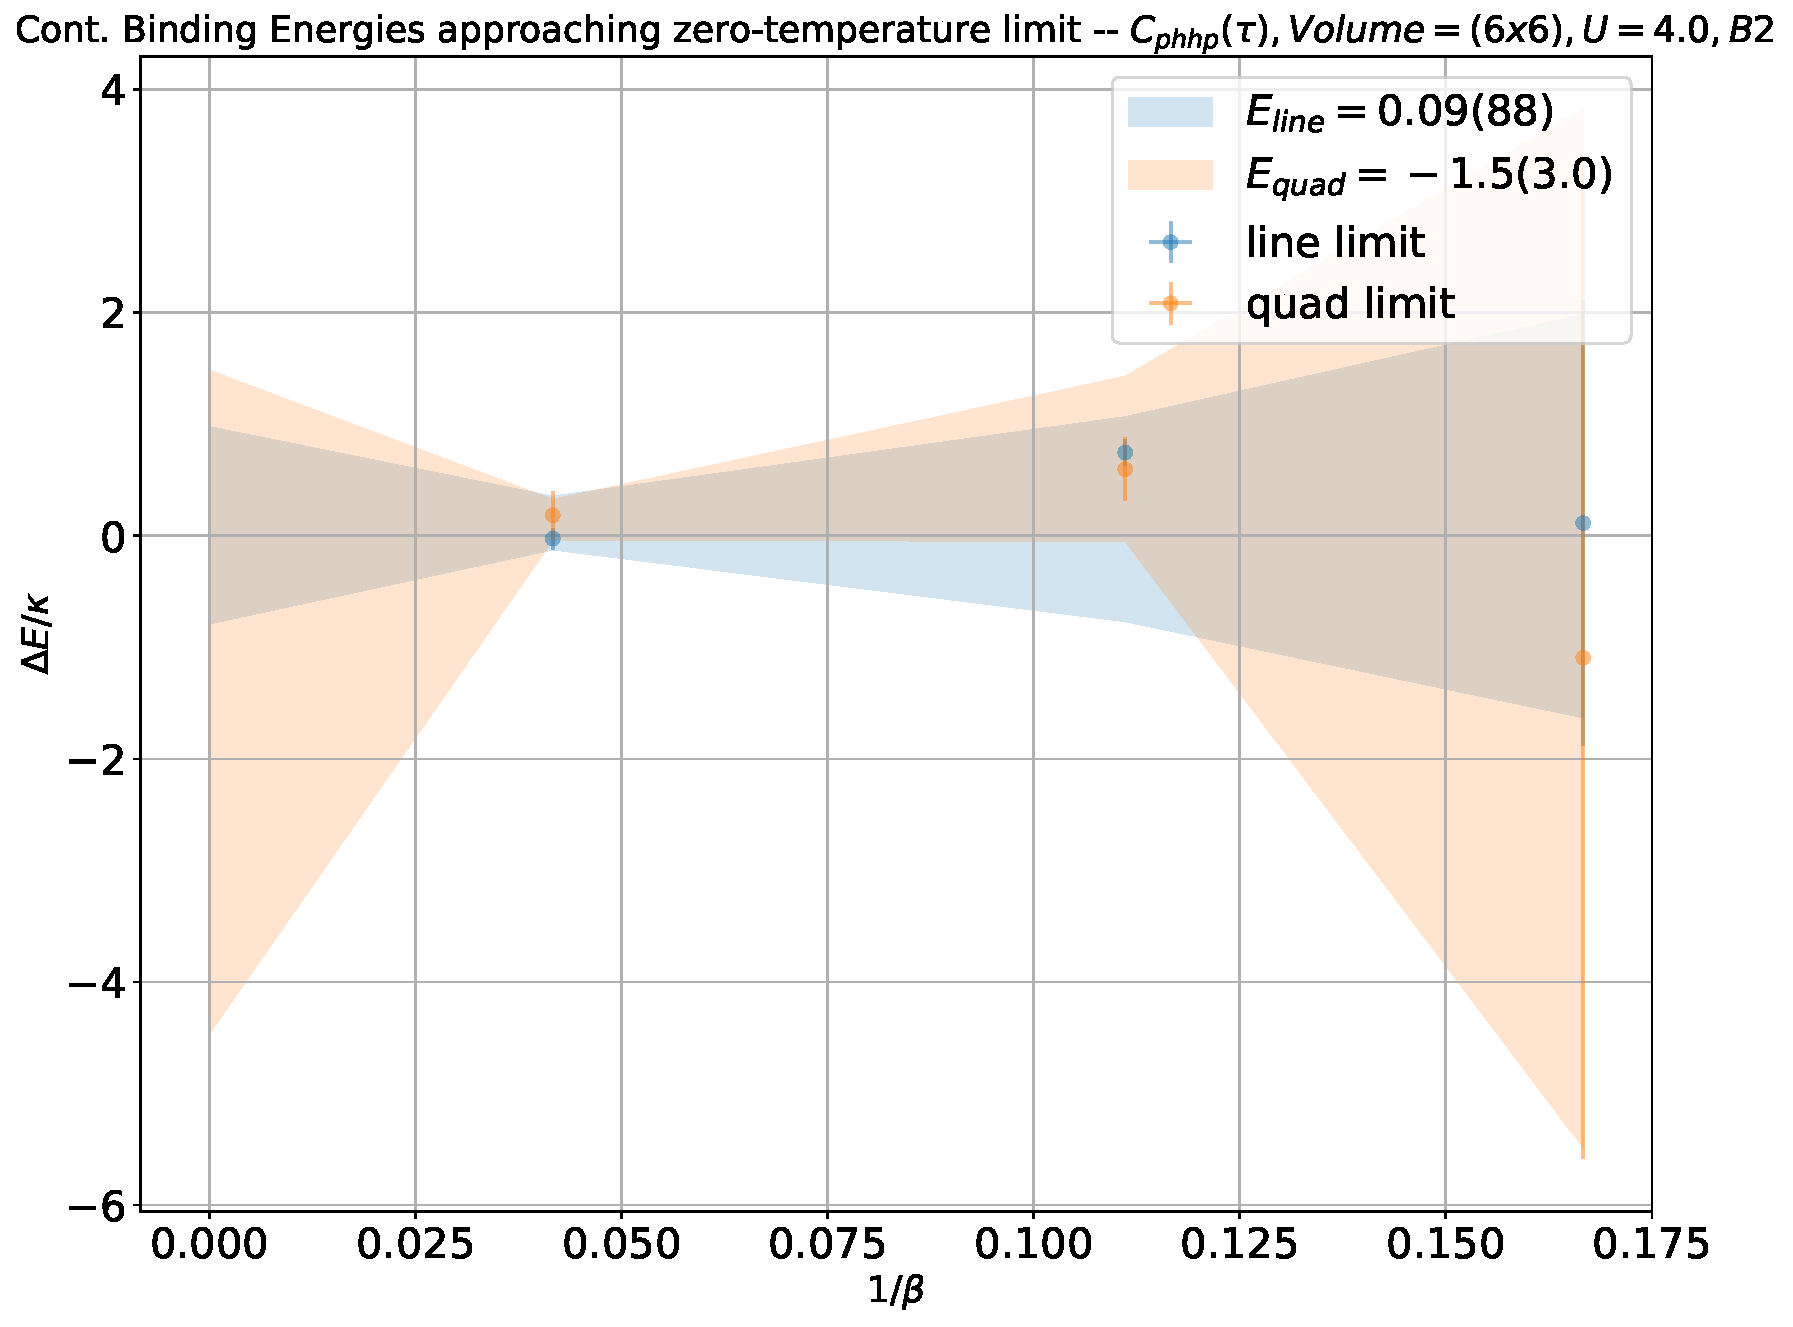
\includegraphics[width=\linewidth]{phhp-0-B2_6x6_U4.0_B24.0_temp.pdf}
      \caption{1b}
      \label{fig:sfig2}
    \end{subfigure}
    \begin{subfigure}{.5\textwidth}
        \centering
        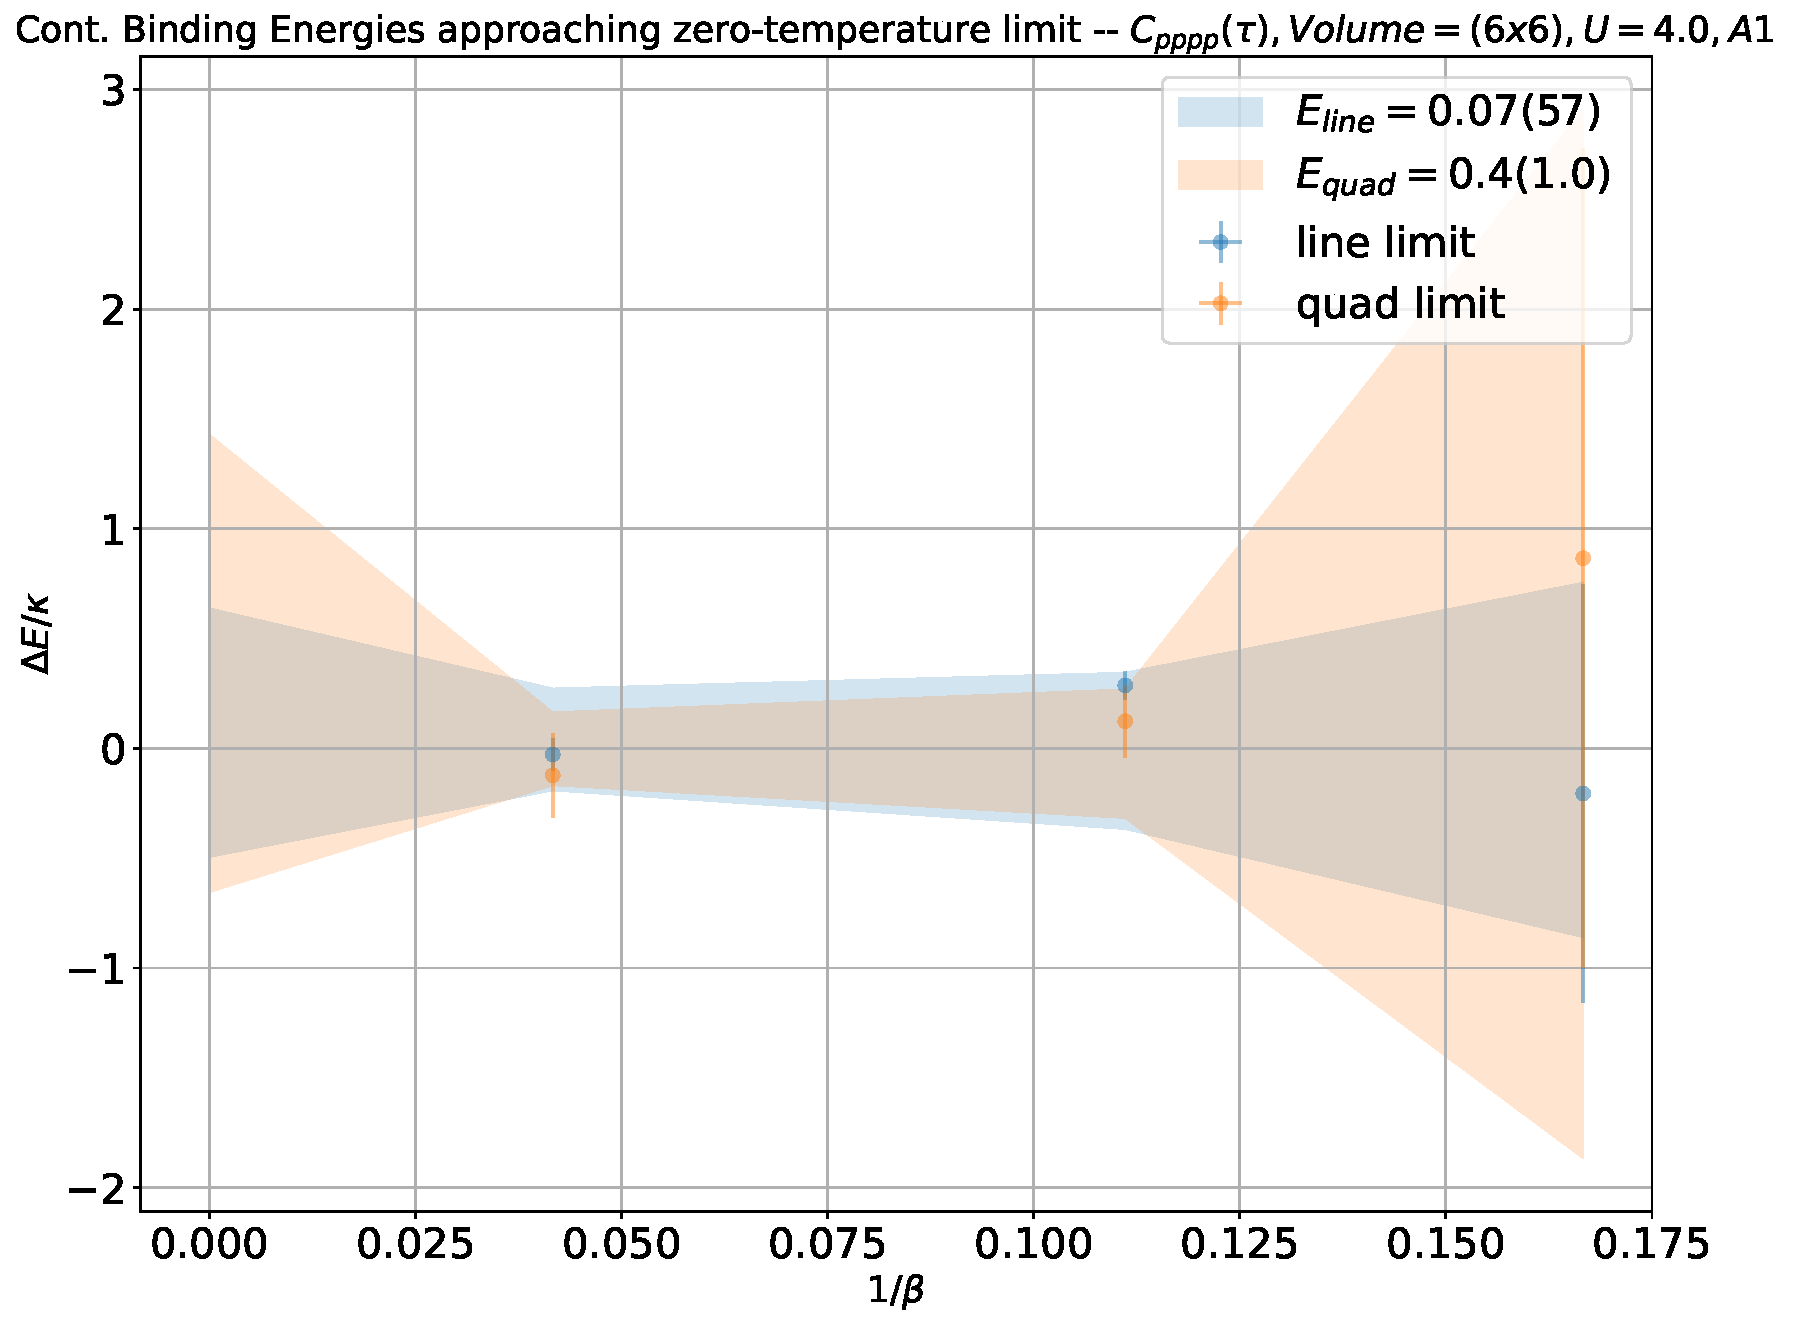
\includegraphics[width=\linewidth]{pppp-0-A1_6x6_U4.0_B24.0_temp.pdf}
        \caption{1c}
        \label{fig:sfig3}
    \end{subfigure}
    \begin{subfigure}{.5\textwidth}
        \centering
        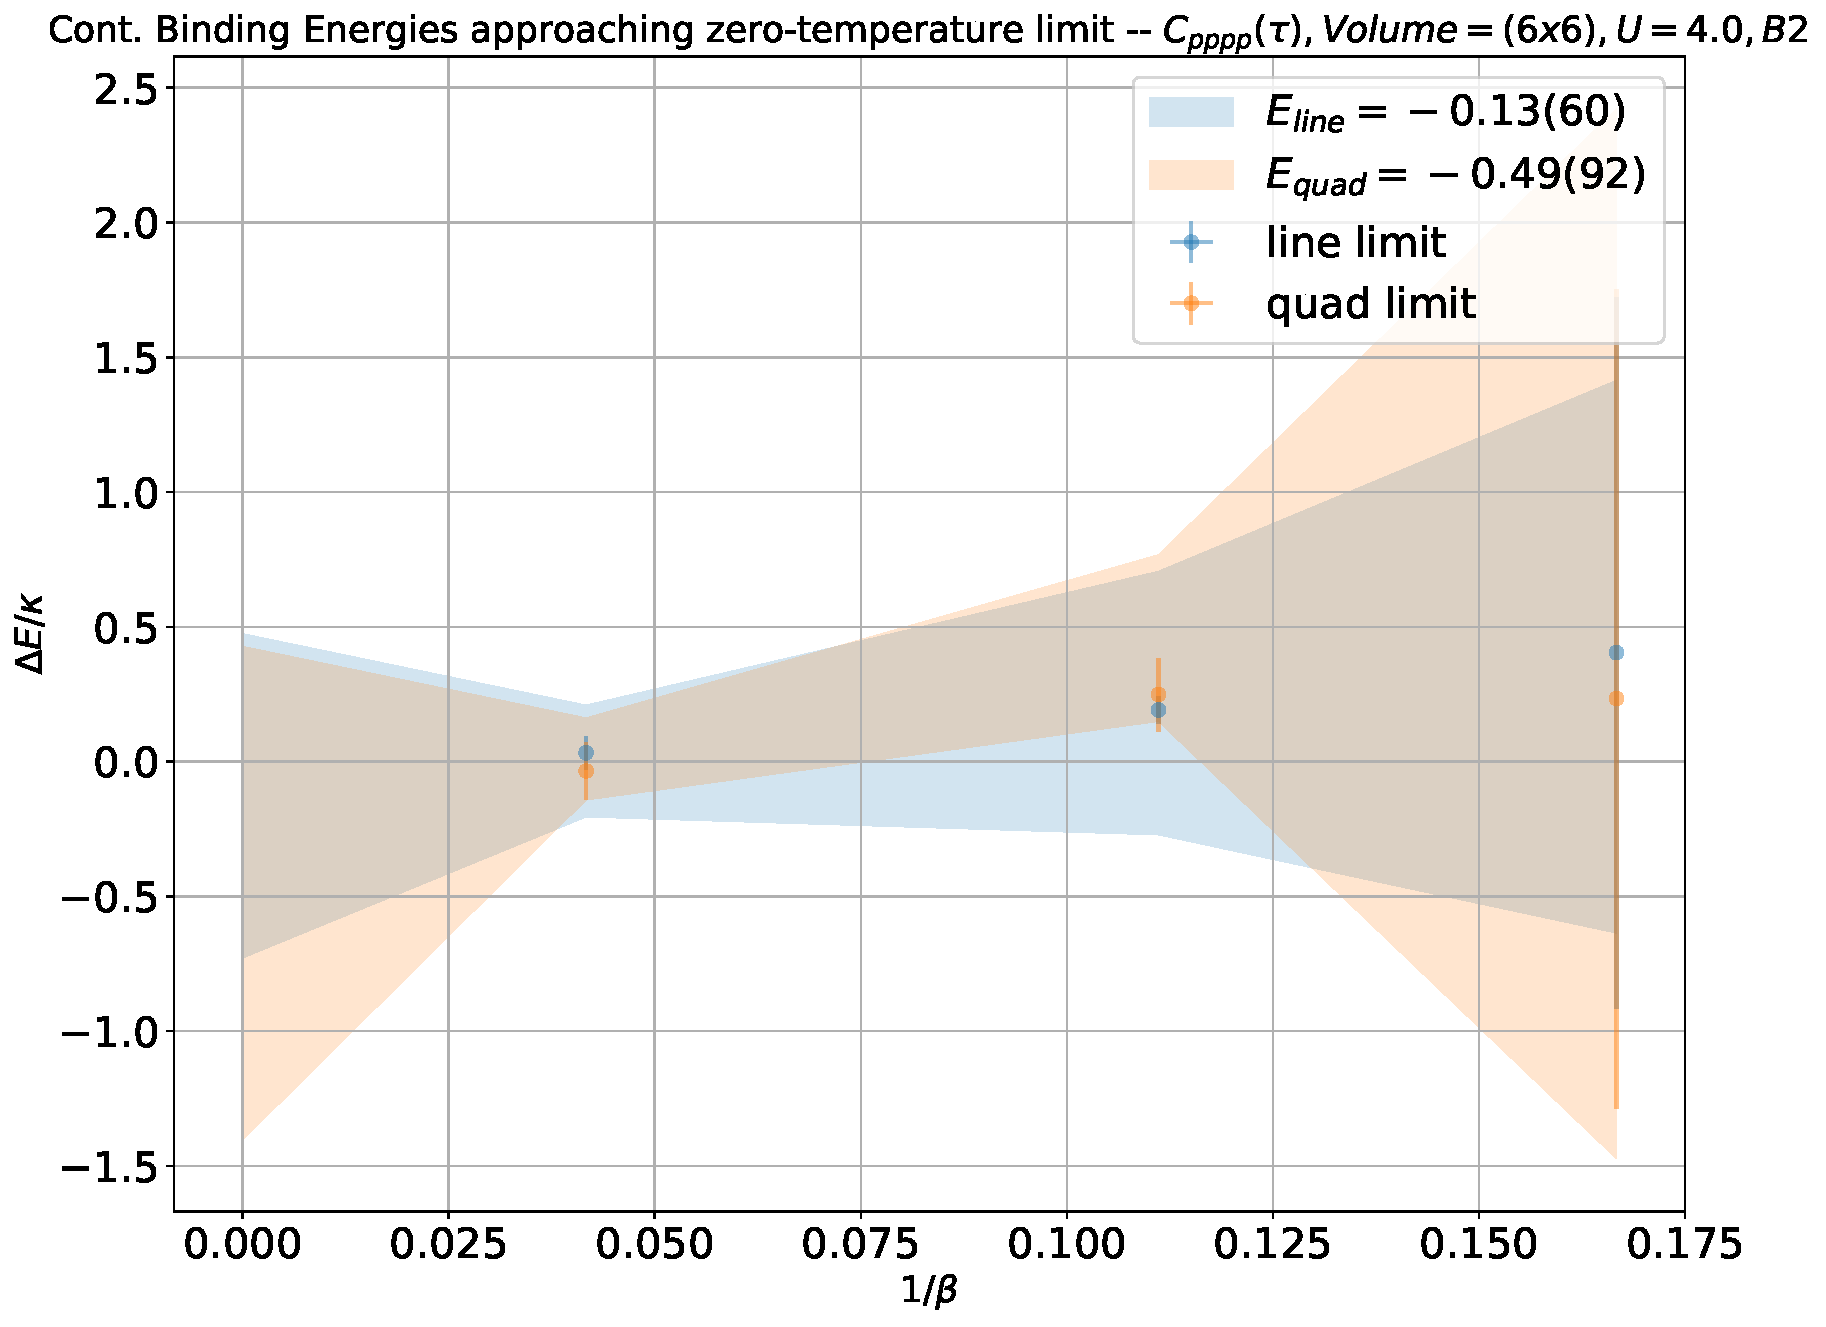
\includegraphics[width=\linewidth]{pppp-0-B2_6x6_U4.0_B24.0_temp.pdf}
        \caption{1d}
        \label{fig:sfig4}
    \end{subfigure}
    \caption{plots of....}
    \label{fig:u4temp}
  \end{figure}
When above the critical coupling ($U=4.0$), the binding energy of the particle-hole pair is negative for $A1$, but not $B2$. 

% If the results from both methods are equivalent up to the statistical uncertainties, we can be confident of our findings. There may be some interesting physics happening that will need further investigation. If the energies are different up to statistical error (that is, what we would expect), this may be due to the fact that the data obtained from the simulations or the model itself have strong intrinsic correlation that are not accounted in the first method.

% The fit of the data is done with a general cosine hyperbolic function. This is because we have symmetrized the functions. Working with the data shown in Table \ref{tab:work_ensembles}, we fit each lattice size independently, as we first need to reach the continuum limit for each lattice configuration and then extrapolate to the infinite volume limit. Results are performed. The results are done only for a total momentum $\Gamma$ and particle momenta $K,K'$.

% We calculate the binding energy (\ref{eq:binding_energy}) of the exciton by first extracting the energy from the two-body correlation function, then the energies of the one-body correlators. After a subtraction, we get $\epsilon$. 

% The next figures show the fitting of the correlators. As our data is symmetrized, we can fit a general cosine hyperbolic function instead of an exponential function. (PRE-REPHRASED)
